% Working manuscript shell for Energy Reports.
% Based on the official Elsevier elsarticle bundle downloaded to
% paper/templates/elsevier-elsarticle/.
% Before submission, re-check the journal Guide for Authors and the current
% Editorial Manager instructions.

\documentclass[preprint,12pt]{elsarticle}

\usepackage{amssymb}
\usepackage{amsmath}
\usepackage{booktabs}
\usepackage{siunitx}
\usepackage{array}
\usepackage{calc}
\usepackage[hidelinks]{hyperref}
\setlength{\emergencystretch}{3em}

\providecommand{\tightlist}{}
\providecommand{\real}[1]{#1}
% Single-symbol wrappers preserve bibliographic diacritics while remaining
% compatible with BibTeX's 8-bit processing path.
\DeclareRobustCommand{\?}[1]{\u{#1}}
\DeclareRobustCommand{\>}[1]{\c{#1}}

\journal{Energy Reports}

\begin{document}

\begin{frontmatter}

\title{Reserve--SOC supervisory energy management for grid--diesel--battery drilling rig power systems under forecast uncertainty}

\author[aff1,aff2]{Shixing Zhang\fnref{equal}\corref{cor1}}
\ead{shixingzhang@cnpc.com.cn}
\author[aff1,aff2]{Pengchong Wei\fnref{equal}}
\author[aff1,aff2]{Lei Luo}
\author[aff1,aff2]{Pengfei Zhang}
\author[aff1,aff2]{Xingjun Yu}
\fntext[equal]{Shixing Zhang and Pengchong Wei contributed equally to this work and share first authorship.}
\cortext[cor1]{Corresponding author.}

\affiliation[aff1]{organization={Baoji Oilfield Machinery Co., Ltd.},
            addressline={Weiyang District},
            city={Xi'an},
            postcode={710016},
            state={Shaanxi},
            country={China}}

\affiliation[aff2]{organization={CNPC National Oil and Gas Drilling Equipment Engineering Technology Research Center Co., Ltd.},
            addressline={Weiyang District},
            city={Xi'an},
            postcode={710016},
            state={Shaanxi},
            country={China}}

\begin{abstract}
We evaluate reserve--SOC supervisory model predictive control (RSS) for
grid--diesel--battery coordination during abrupt load transitions. Evaluation
uses a 72 h record and ten independently
generated holdouts from a single mechanistic drilling-load and power-system
simulator; no synchronized measurements from the target rig are used. Seven
online controllers follow a declared comparison protocol; the main contrasts
use rule-based control (RB), deterministic margin-loaded
reference MPC (MLR), and an independently implemented causal full-MILP (CR).
RSS records 813.43 kWh of unserved energy, compared with 840.96 kWh for RB,
906.04 kWh for MLR, and 1,165.81 kWh for CR. These reductions are
3.27\%, 10.22\%, and 30.23\%, with Holm-adjusted exact sign-flip $p$-values of
0.02, 0.01, and 0.01. Risk-adjusted cost, a shortage-dominated composite rather
than independent economic evidence, falls by 3.85\% relative to RB and 9.34\%
relative to MLR. CR uses one point forecast without the forecast-error envelope
or reserve--SOC supervisor. Because CR is weaker than RB under
this protocol, the 30.23\% RSS--CR gap is interpreted as a bundled boundary
comparison, not an isolated component effect. Component interventions associate
SOC supervision with a 2.86--4.11 kWh mean per-holdout reduction and the
forecast-envelope bundle with a further 2.12 kWh reduction. An auxiliary raw
evidential risk interface improves selected classification metrics but worsens
the Brier score and does not change unserved energy. These findings are limited
to the simulated system and do not establish performance for the target rig or
drilling rigs generally.
\end{abstract}

\begin{highlights}
\item Evidence uses one mechanistic simulator; no target-rig measurements.
\item Seven online controllers follow the declared simulation and audit protocol.
\item RSS cuts unserved energy 3.27\% vs RB and 10.22\% vs MLR.
\item Composite risk-adjusted cost falls 3.85\% vs RB; it is shortage-dominated.
\item CR is an independent point-forecast MILP, not a component ablation.
\end{highlights}

\begin{keyword}
drilling rig power system \sep multi-source energy management \sep battery energy storage \sep model predictive control \sep unit commitment \sep supply reliability
\end{keyword}

\end{frontmatter}

% Keep the body separate so the Markdown remains the author-facing source.
\section{Introduction}\label{introduction}

Drilling rigs are energy-intensive industrial systems whose electrical
demand changes sharply with operating state. Drilling, circulation,
connection, tripping, and auxiliary activities impose different demand
levels and different transition dynamics. When a rig is supplied by a
weak grid connection, diesel generator units, and a battery energy
storage system (BESS), the operating problem involves more than reducing
energy cost. The controller must also maintain power balance, respect
generator commitment and ramping constraints, preserve sufficient
storage state of charge (SOC), and protect high-priority loads when
available supply becomes insufficient.

This problem has a direct operational consequence. A controller that
reacts only to instantaneous load may discharge the BESS before a
transition, or may start too many diesel units and replace relatively
inexpensive grid power with fuel consumption. Conversely, a controller
that focuses only on economic dispatch may leave insufficient reserve
for a short high-power event. The resulting trade-off is particularly
important for drilling rigs because their load profile combines
sustained operation with short, high-amplitude transitions.

Energy management studies have investigated hierarchical scheduling,
multi-objective microgrid dispatch, energy storage coordination, and
model predictive control (MPC). For example, bilevel energy management
has been used to coordinate security, reliability, storage, and
demand-side management
\citep{jokar2022bilevel},
while predictive energy management has been applied to hybrid vessel
grids \citep{vafamand2020predictive}. Stochastic and random-setting formulations have also been used
for isolated hybrid microgrids with diesel generation and storage
\citep{vergine2022optimal}.
These studies establish the value of combining forecasting, uncertainty
representation, and constrained optimization. They also motivate a
system-level evaluation that reports drilling-load transitions, discrete
multi-generator commitment, storage protection, and emergency load
prioritization under one declared protocol.

The closest drilling rig precedent considered rule-based generator
scheduling together with battery storage for diesel power-plant
fuel-efficiency improvement
\citep{pavkovic2016oil}. This prior work motivates the present application, but it also
sets a clear comparison requirement: the contribution cannot be reduced
to using a BESS in a drilling rig. The relevant question is whether
forecast uncertainty and supply risk can be transferred into a
controller that remains physically feasible while avoiding unnecessary
generator commitment.

This paper develops a reserve--SOC supervisory energy-management framework
for a grid--diesel--battery drilling rig power system. The framework links
short-horizon load forecasting to scenario-based conditional value-at-risk
(CVaR) dispatch, discrete generator commitment, storage reserve management,
and priority-based load protection. It addresses three questions: whether the
integrated controller changes supply reliability and the associated composite
cost, which prespecified component interventions are associated with changes in
physical dispatch, and whether the resulting schedules satisfy the stated
physical and computational constraints. The
paper makes four contributions:

\begin{enumerate}
\def\labelenumi{\arabic{enumi}.}
\tightlist
\item
  We define and audit a causal information boundary that admits only current
  measurements, executed equipment history, and forecasts available at the
  decision time, while excluding future true load and future-derived state
  flags.
\item
  We use declared component-level interventions to estimate
  intervention-specific changes associated with the risk input, the
  reserve--SOC supervisor, and the implemented forecast-envelope bundle under
  their declared fixed comparison settings.
\item
  We implement an independent causal rolling full-MILP comparator that shares
  the realized plant state and cost terms but uses a single point forecast and
  omits both the forecast-error envelope and reserve--SOC supervisor; it is
  therefore a bundled boundary comparator rather than a component ablation.
  Under this protocol, CR has higher unserved energy than RB; this difference
  cannot be attributed to any single component.
\item
  We evaluate seven online controllers over ten independently generated
  simulation holdouts, using seed-level statistics and physical feasibility
  checks, while reserving the main inferential contrasts for RB, MLR, and CR.
  The 72 h record and all holdouts are generated by a single mechanistic
  simulator; no synchronized target-rig measurements are used, and the
  conclusions are limited to this simulated system.
\end{enumerate}

The evaluation comprises a 72 h load replay for forecasting and ten
independently generated holdouts for the primary dispatch comparison. Separate
holdout groups are used for the auxiliary risk interface.
Section~\ref{system-boundary-and-data} describes the data provenance and the
scope of the resulting conclusions.

\section{Related work}\label{related-work}

\subsection{Drilling rig and industrial hybrid power systems}

Energy storage has been studied in drilling rig power systems as a means of
reducing diesel generator inefficiency and smoothing fast load changes.
Pavkovi\'{c} et al. combined rule-based generator scheduling with a BESS for
an oil-drilling diesel power plant \citep{pavkovic2016oil}. A separate review
of drilling rig storage systems discusses the operating and sizing role of
storage in drilling applications \citep{chupin2021drillingstorage}. For
offshore drilling, Huang et al. formulated generation scheduling with
uncertain renewable generation and uncertain platform loads
\citep{huang2019drilling}. These studies establish the application relevance
of coordinated generation and storage. Adjacent offshore studies also assess
diesel-electric dispatch with BESS integration using field data
\citep{peixoto2024psv} and integrated management of offshore oil-and-gas
systems with renewable generation and gas turbines \citep{banihabib2023offshore}.
Building on this foundation, the present work connects causal short-horizon
forecasting, finite-ensemble shortage risk, discrete multi-unit commitment, SOC
supervision, and priority-based protection in one reproducible controller
evaluation.

\subsection{Microgrid energy management and supervisory control}

The broader microgrid literature provides the conceptual foundation for
hierarchical supervisory control and energy management. Reviews have
classified storage control, microgrid supervisory controllers, and the
optimization methods used by energy management systems
\citep{zamora2010controls,meng2016supervisory,zia2018microgrid}. A recent
review further organizes energy-management strategies by their treatment of
forecasting, uncertainty, optimization, and control objectives
\citep{abbasi2023emsreview}. Application-specific studies include bilevel
security and reliability coordination \citep{jokar2022bilevel} and random
setting management of isolated hybrid microgrids
\citep{vergine2022optimal}. More recent work covers BESS and renewable-resource
coordination \citep{onsomu2024bessreview}, affordability--flexibility--security
trade-offs \citep{pamulapati2023trilemma}, MPC-based EMS design
\citep{joshal2023mpcreview,hu2024empc}, two-level economic MPC
\citep{vivas2025hierarchical}, and a two-layer robust MPC that exchanges
prediction-error-interval information between control time scales
\citep{lim2026twolayer}. This body of work supports the use of a layered
architecture, but the reported results are often organized around a single
microgrid formulation or controller. Our distinction is the explicit audit
boundary between forecasting, dispatch, SOC mode selection, and emergency
load prioritization, together with a declared causal information set and
component-level interventions.

\subsection{MPC, MILP, and risk-aware scheduling}

MPC is well suited to storage-constrained operation because it repeatedly
updates decisions as state measurements and forecasts change; a dedicated
review surveys MPC architectures and implementation issues for microgrids
\citep{hu2021mpcoverview}. Mixed-integer predictive scheduling has been used
to account for storage impacts and forecast uncertainty
\citep{zhang2015smartmicrogrid}, while distributed predictive controllers
have coordinated multiple microgrids and hybrid storage systems
\citep{dao2019hierarchical,garciatorres2019network}. Resilience-oriented MPC
also makes reserve and supply continuity explicit in the scheduling problem
\citep{tobajas2022resilience}. In parallel, stochastic MILP has been used for
hybrid-microgrid energy management \citep{franke2020stochasticmilp}, and
robust cost--risk scheduling has incorporated worst-case CVaR
\citep{ji2018robustcvar}. The CVaR construction used here follows the
standard auxiliary-threshold formulation of Rockafellar and Uryasev
\citep{rockafellar2000cvar}. Recent studies further report economic and
multi-objective MPC \citep{vasquez2023mpcmultiobjective}, systematic
MPC-EMS design \citep{pajares2023mpcmethodology}, and BESS-integrated
predictive control with experimental evaluation
\citep{sepehrzad2023dcmicrogrid}. Scenario-based stochastic MPC
\citep{alarcon2023scenariompc}, risk-aware stochastic control
\citep{tereza2023riskaware}, and distributionally robust CVaR scheduling
\citep{zhang2023drcvar} show complementary ways to represent uncertainty.
Our contribution is the application-specific reserve--SOC coupling of these
tools, supported by component interventions and an independently implemented
bundled causal full-MILP boundary comparator.

\subsection{Evidence fusion for uncertain decisions}

Belief-function methods represent source conflict and residual ignorance in
addition to class support. Yager's rule transfers conjunctive conflict to the
full frame of discernment \citep{yager1987dempster}, while pignistic
transformation supports decisions without treating epistemic imprecision as
an ordinary probability \citep{denoeux2019decision}. Power-system applications
have used evidence fusion for transformer and post-fault network diagnosis
\citep{demirci2022transformer,wu2024distribution}, and recent work shows that
basic-probability-assignment design materially affects diagnostic performance
\citep{guan2025optimized}. We use evidence fusion only as an auxiliary
risk-reporting interface and evaluate its classification and dispatch effects
separately from the primary controller.

\subsection{Resilience and priority-based critical-load protection}

Priority-aware management is a related but distinct decision layer: it
allocates a constrained supply to loads with different service importance,
rather than establishing that the total supply shortage has been removed.
Recent work combines demand and generation prediction with critical-load
management \citep{esmaeili2023critical}, formulates real-time optimization
for priority-weighted load restoration \citep{erenoglu2023restoration}, and
studies resilient scheduling under uncertain demand and storage resources
\citep{niknami2024resilient}. Hybrid switched MPC with demand-side management
also illustrates why supervisory mode selection and controllable demand must
be stated separately \citep{maslak2024switchedmpc}. Accordingly, the present
paper reports priority protection as a diagnostic allocation result and does
not infer improved total supply adequacy from the protection-mode flag.

\subsection{Short-horizon load forecasting}

The forecasting comparison spans naive, tree-based, recurrent,
convolutional, and transformer-based candidates. Temporal Fusion
Transformers provide an interpretable multi-horizon forecasting design
\citep{lim2021tft}; PatchTST uses patch-based transformer representations
for long-term time-series forecasting \citep{nie2023patchtst}; and
iTransformer reorients the transformer representation for multivariate
forecasting \citep{liu2024itransformer}. A recent review identifies deep
learning choices, online robustness, and feasibility as central concerns for
short-term load forecasting \citep{eren2024stlfreview}. The broader
transformer lineage includes efficient sparse attention
\citep{zhou2021informer}, decomposition and autocorrelation
\citep{wu2021autoformer}, frequency-enhanced decomposition
\citep{zhou2022fedformer}, and general temporal-variation modeling
\citep{wu2023timesnet}. These methods provide strong forecasting baselines.
We report their prediction performance separately and then evaluate how
forecast errors propagate into generator commitment and storage decisions.

\subsection{Position of the present study}

The individual ingredients of the proposed framework are established in prior
work. The systems question addressed here is how forecast uncertainty, generator
commitment, storage reserve, and load priority should interact during rapid
drilling-load transitions. We address this question under a common plant,
realized-trace, cost, solver, and audit boundary; controller-specific forecast
representations, scenario constructions, and terminal-SOC rules are declared
explicitly. Ten primary holdouts support the controller comparison;
prespecified interventions estimate local changes associated with the forecast-
envelope bundle and SOC supervisor; and an independently implemented causal
full-MILP provides a bundled causal optimization boundary reference. The auxiliary
evidence-fusion study is reported separately because recognition quality does
not necessarily translate into a change in physical dispatch.

\section{System boundary and data}\label{system-boundary-and-data}

\subsection{System boundary}\label{system-boundary}

The system contains four functional components: (i) an external grid
connection with time-varying available capacity, (ii) a set of diesel
generator units, (iii) a BESS with power and SOC limits, and (iv) an
electrical load representing the drilling rig and auxiliary equipment.
The controller receives measurements and causally available state
information. It produces a receding-horizon plan and applies the first
control action before the next measurement update.

The load is partitioned into critical, essential, and interruptible classes
for evaluating priority-based protection when available supply is
insufficient. The class proportions are control-study settings; deployment
values must be approved through the drilling rig's electrical and safety
procedures.

The implementation uses a 5 s sampling interval for the main
high-frequency data path. The forecast task uses a 10 min history to
predict the following 1 min horizon. The dispatch controller operates on
the forecast package and current equipment state; all future true load
and future-derived operation-state flags are excluded from online
features.

\subsection{Evaluation data}\label{evaluation-data}

The evaluation dataset contains a 72 h active-power record sampled at 5 s,
with 51,840 timestamped rows and 51,827 rows after quality processing. It is
generated by a mechanistic drilling-load and multi-source power-system
simulation parameterized from public process and equipment evidence. The
dataset contains total load, operating state, available supply, generator
status, battery power, and SOC.

The load generator is a finite-state semi-Markov simulation. If $Z_j$ is the
operating state of segment $j$, then its duration is drawn as
$D_j\sim\mathcal U(a_{Z_j},b_{Z_j})$ and the next state is drawn from the fixed
categorical transition row $T_{Z_j,:}$. The duration ranges in minutes are
idle 12--45, circulation 25--100, drilling 20--70, connection 5--12, tripping
35--180, and maintenance 20--90. The nonzero transition probabilities are:
idle to circulation/drilling/tripping/maintenance, 0.45/0.10/0.25/0.20;
circulation to drilling/idle/tripping/maintenance, 0.65/0.15/0.10/0.10;
drilling to connection/circulation/tripping/idle, 0.62/0.23/0.07/0.08;
connection to drilling/circulation/tripping/idle, 0.82/0.12/0.02/0.04;
tripping to circulation/idle/maintenance, 0.50/0.30/0.20; and maintenance to
idle/circulation, 0.70/0.30.

Within a segment, physical load is
\begin{equation}
\label{eq:simulated-load}
P_t=P^{aux}_t+P^{mud}_t+P^{top}_t+P^{draw}_t+P^{other}_t,
\end{equation}
where each component combines a state-specific rated-power fraction, a
periodic or triangular operating term, and a Gaussian innovation; drilling
terms are additionally modulated by simulated depth and formation hardness.
All components within each state are rescaled by one frozen factor to the
public-evidence target mean and then constrained by the declared state cap.
The recorded power channel is
\begin{equation}
\label{eq:simulated-measurement}
Y_t=Q_{0.5}\!\left(\operatorname{clip}\{P_t(1+r_t),180,2000\}\right),\qquad
r_t=\operatorname{clip}\{w_t+b_t,-0.025,0.025\},
\end{equation}
where $w_t$ is Gaussian white relative error with standard deviation 0.005,
and $b_t$ is a Gaussian-innovation AR(1) relative drift with coefficient
0.9995 and standard deviation 0.003. A daily Bernoulli trial with probability
0.35 introduces a missing block whose start is uniform within the day and
whose duration is discrete uniform from 15 to 90 s; these short gaps are
linearly interpolated.

The frozen calibration map records a source identifier and provenance class
for each state-load target, equipment quantity, and cost field. Public drilling
generator and storage observations anchor the fleet and BESS ranges
\citep{pavkovic2016oil,chupin2021drillingstorage}; state means and caps are
mapped to the corresponding public load sources in the calibration file.
Transition probabilities, duration ranges, generator ramp and dwell settings,
startup and degradation costs, and the missingness model are marked as
engineering scenario assumptions rather than distributions fitted to the
target rig. Exact state-specific coefficients and transformations are fixed in
the versioned generator and resolved configuration retained with the
reproducibility artifacts. Calibration reads neither forecasts nor controller
outcomes.

The forecasting replay contains 51,709 samples, of which 51,697 are scored.
A fixed chronological split is used for model comparison. The power scaler
is fitted on the training partition, ensemble weights and forecast-error
settings use the validation partition, and the test targets are excluded from
model fitting and selection.

For dispatch, each forecast origin retains one 12-step prediction row for
each model. The seven-member scenario package consists of Persistence,
Validation-Weighted-Ensemble (VWE), PatchTST, iTransformer,
StateAware-TCN-Attention, StateAware-Patch-Transformer, and
StateAware-DualBranch-Patch-Transformer. Persistence repeats the last observed
load over all 12 steps. VWE is a nonnegative convex combination of XGBoost,
LSTM, TCN, and the three state-aware models; its weights sum to one and are
fitted on validation data by minimizing mean squared error plus an
$L_2$ penalty of $10^{-4}$. The other five members enter the package as their
direct multi-step outputs. Test targets are not used to construct or weight
these members.

An official public Wellsite Information Transfer Standard Markup Language
(WITSML) example provides the drilling process and state-signal schema used in
the interface design. Because the example does not contain synchronized total
active power, it is not included in the controller-performance evaluation.

Figures~\ref{fig:load-feature-summary} and~\ref{fig:operating-state-curves}
summarize the load features and representative operating-state curves used to
define the forecasting and dispatch problem; Table~\ref{tab:evaluation-datasets}
summarizes the evaluation datasets and their roles.

\begin{figure}
\centering
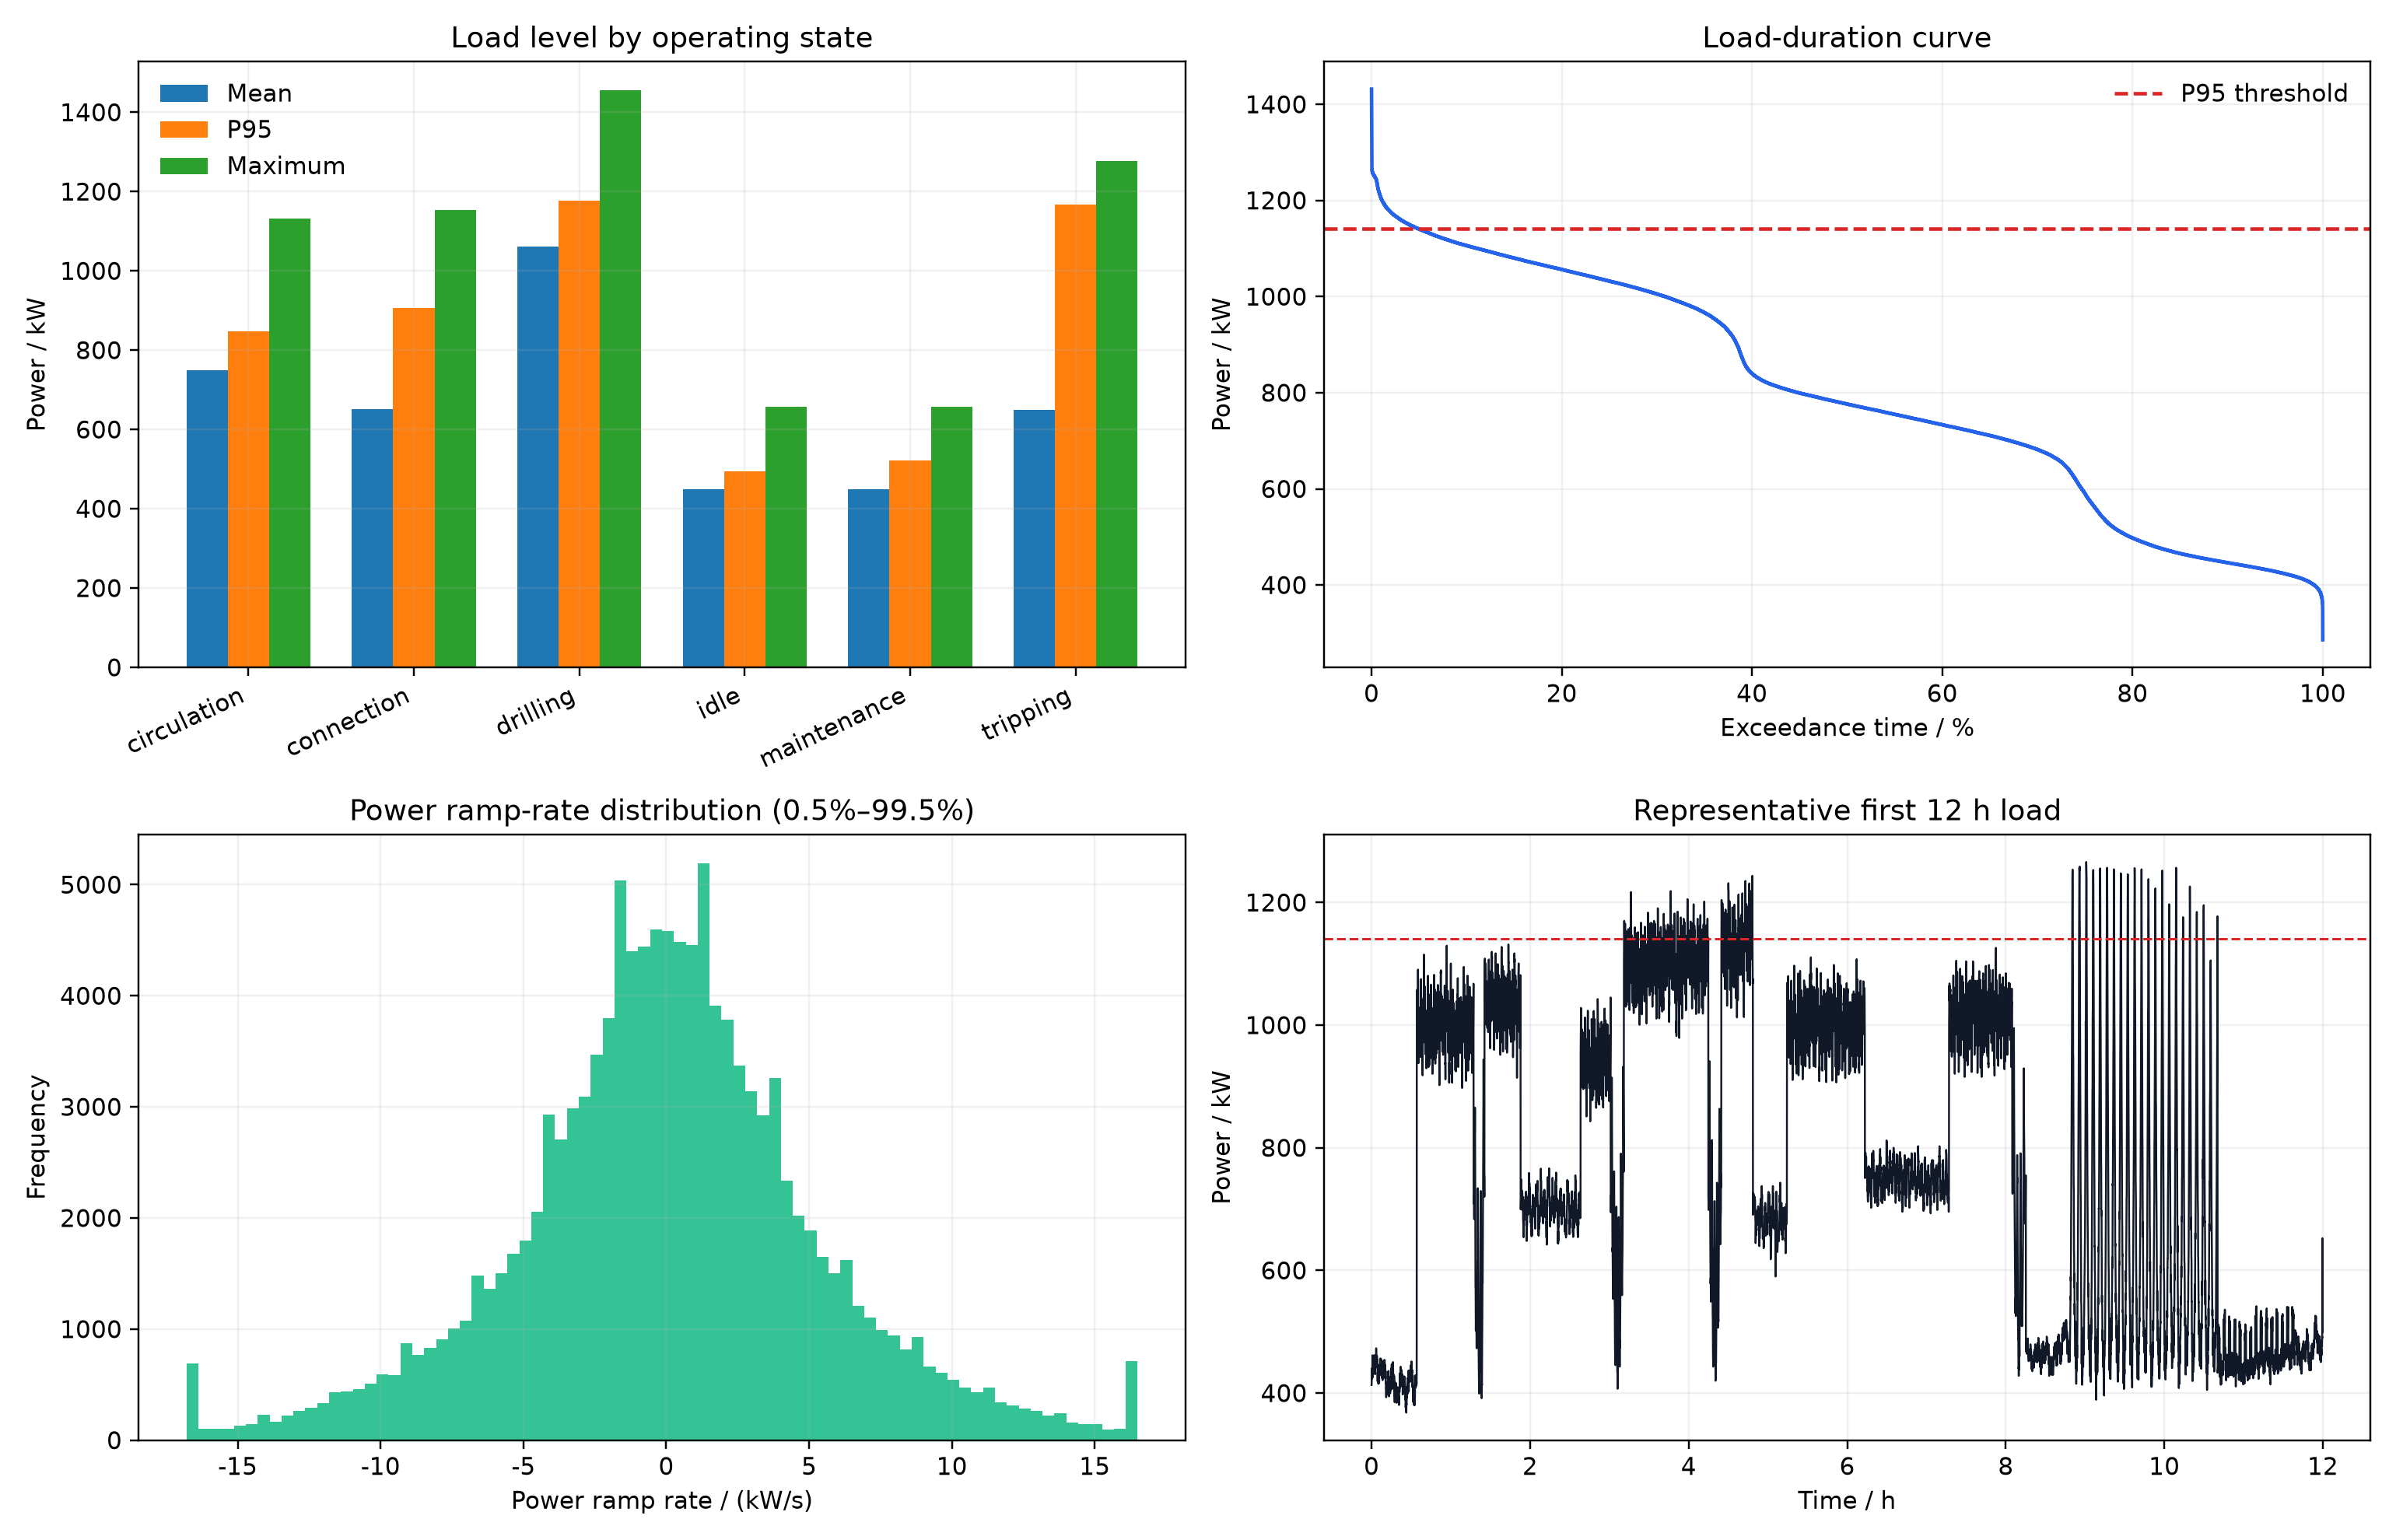
\includegraphics[width=\linewidth,keepaspectratio]{../figures/fig02_load_feature_summary_en.png}
\caption{Load-feature summary across operating states and representative
intervals}
\label{fig:load-feature-summary}
\end{figure}

\begin{figure}
\centering
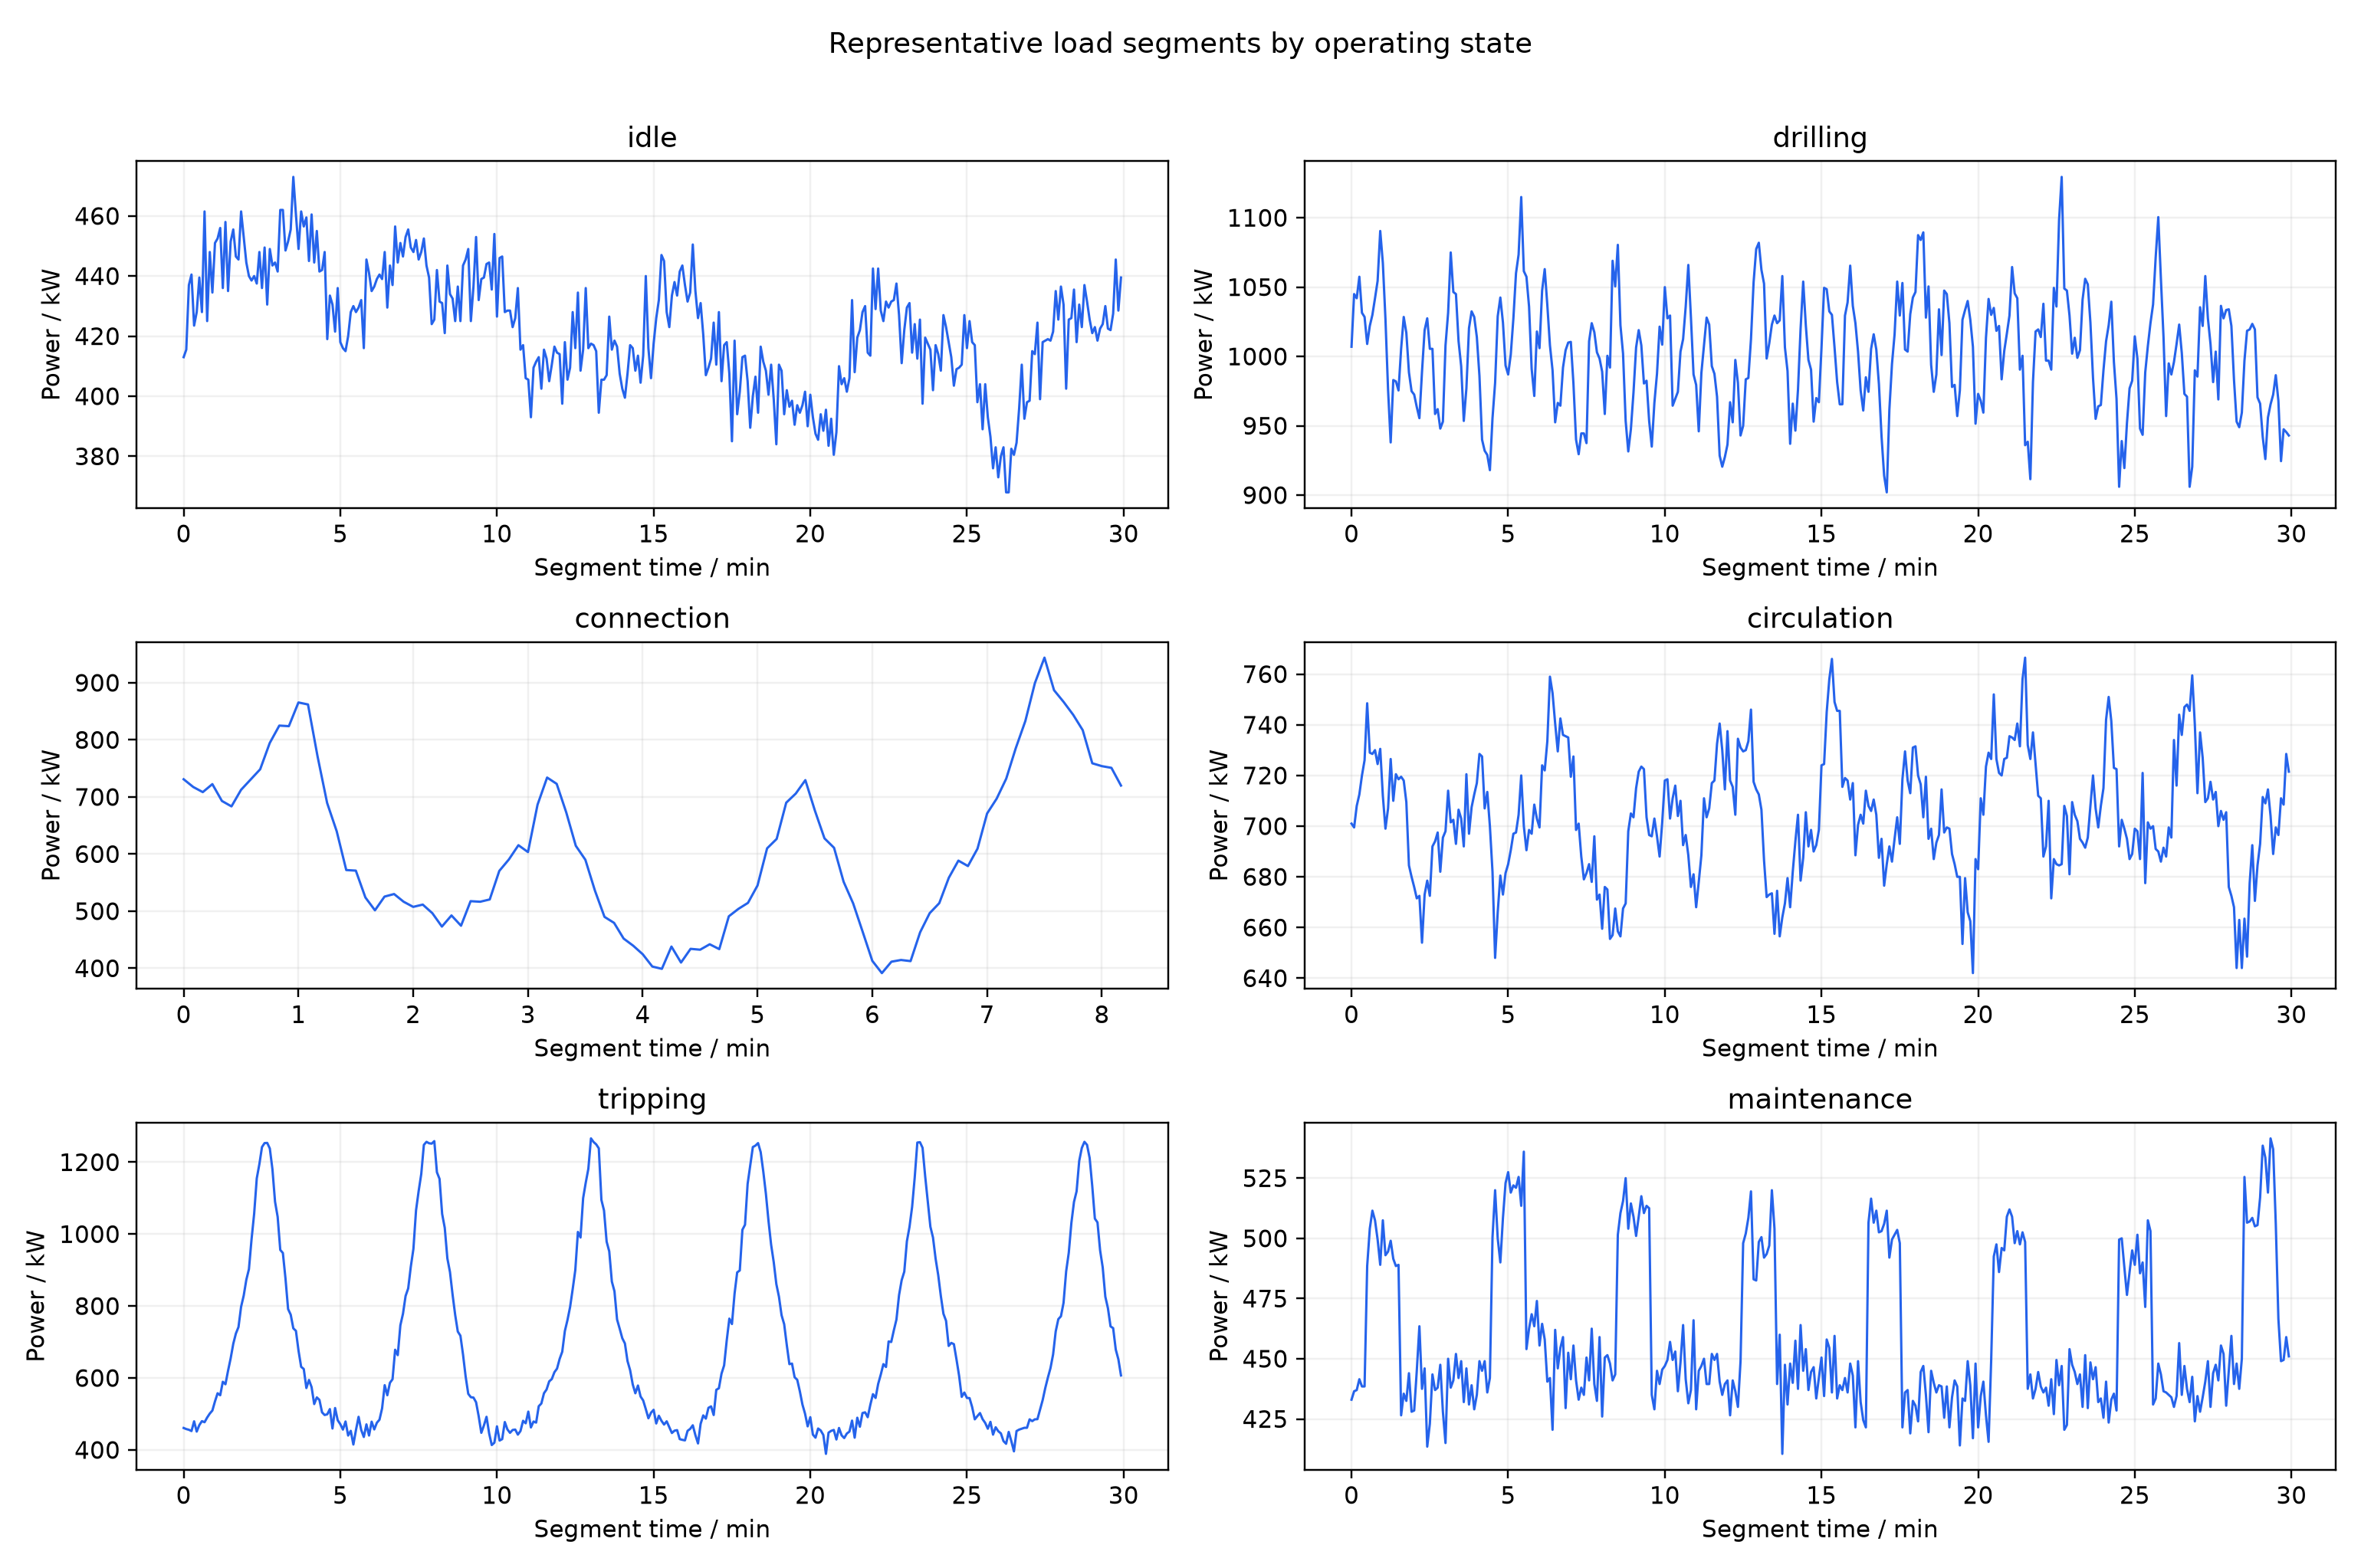
\includegraphics[width=\linewidth,keepaspectratio]{../figures/fig03_typical_state_curves_en.png}
\caption{Representative load curves for six drilling operating states}
\label{fig:operating-state-curves}
\end{figure}

\begin{table}[!t]
\caption{Evaluation datasets and their roles}
\label{tab:evaluation-datasets}
\centering
\footnotesize
\begin{tabular}{@{}
  >{\raggedright\arraybackslash}p{(\linewidth - 6\tabcolsep) * \real{0.21}}
  >{\raggedright\arraybackslash}p{(\linewidth - 6\tabcolsep) * \real{0.20}}
  >{\raggedleft\arraybackslash}p{(\linewidth - 6\tabcolsep) * \real{0.17}}
  >{\raggedright\arraybackslash}p{(\linewidth - 6\tabcolsep) * \real{0.42}}@{}}
\toprule
\begin{minipage}[b]{\linewidth}\raggedright
Dataset / source
\end{minipage} & \begin{minipage}[b]{\linewidth}\raggedright
Role
\end{minipage} & \begin{minipage}[b]{\linewidth}\raggedleft
Resolution
\end{minipage} & \begin{minipage}[b]{\linewidth}\raggedright
Content and provenance
\end{minipage} \\
\midrule
Rig power-system record & Forecasting and dispatch evaluation & 5 s & Load,
supply, generator, storage, operating-state, and risk variables \\
Forecasting replay & Chronological model comparison & 5 s & Fixed train,
validation, and test partitions from the evaluation record \\
Public WITSML example & Process-signal interface design & source-dependent &
Public drilling process and operating-state fields; no synchronized active
power channel \\
\bottomrule
\end{tabular}
\end{table}

\subsection{Preprocessing and
causality}\label{preprocessing-and-causality}

The preprocessing path canonicalizes timestamps, checks the sampling
interval, records quality flags, and imputes only the documented short
gaps. The forecast input window is constructed from information
available at the prediction timestamp. Transition features are based on
history, not on the future operation-state label. This distinction is
essential because a future-derived transition flag would make the
forecast or controller appear stronger while being unavailable during
online operation.

Development cases and holdout cases are separated throughout the evaluation.
Controller settings and eligibility criteria are fixed before holdout outcomes
are inspected, and no parameter is retuned during the ten-case primary
comparison.

For each holdout, its seed initializes the state sequence and durations,
state-specific amplitudes and Gaussian innovations, depth/formation evolution,
transient timing and amplitude, and missing-block process. A deterministic
derived seed, equal to the holdout seed plus 14,000,003, initializes the
post-calibration measurement error. Distinct holdout seeds therefore define
separate pseudorandom realizations of the same frozen simulator; they are not
claimed to be draws from an empirically fitted target-rig population.

All seven member rows at a dispatch decision share the same causal forecast
origin and horizon. Source indices are required to be consecutive before a
dispatch window is selected. For CEF, a test-period residual can update the
error-feedback state only after its complete 12-step target window has been
observed; at forecast origin $i$, the newest eligible residual is therefore
from origin $i-12$. For each holdout, the simulator random-number generator is
initialized with the holdout seed, and the forecasting benchmark initializes
NumPy and PyTorch once with the same seed before fitting models in the fixed
implementation order; XGBoost receives that seed as its random state. The
seven-member stacking and subsequent dispatch introduce no random draw and
are not reseeded by scenario or decision time.

\section{Reserve--SOC supervisory coordination
framework}\label{reserve-soc-supervisory-coordination-framework}

\subsection{Forecasting module}\label{forecasting-module}

Let $L_t$ denote the total active load at time $t$, and let $H$ be the
forecast horizon. The forecasting module produces a point forecast in
Equation~\eqref{eq:point-forecast}.

\begin{equation}
\label{eq:point-forecast}
\hat{\mathbf L}_{t+1:t+H}=f_\theta(\mathbf X_{t-W+1:t}),
\end{equation}

where $W$ is the historical input length and $\mathbf X$ contains the
available load, equipment, and causal process features. The comparison
includes Persistence, XGBoost, long short-term memory (LSTM), temporal
convolutional network (TCN), PatchTST, iTransformer, and state-aware ensemble
variants. The causal error-feedback ensemble supplies the point forecast used
by the controller, while iTransformer provides the strongest forecasting
baseline in the replay \citep{lim2021tft,nie2023patchtst,liu2024itransformer}.

For control, the point forecast is combined with a forecast-error
envelope. In generic form, Equation~\eqref{eq:scenario-forecast} applies.

\begin{equation}
\label{eq:scenario-forecast}
\mathbf L^{(s)}_{t+1:t+H}=\hat{\mathbf L}_{t+1:t+H}+\boldsymbol\epsilon^{(s)}_{t+1:t+H},
\end{equation}

where $s$ indexes members and $\boldsymbol\epsilon^{(s)}$ is the deterministic
difference between member $s$ and the CEF point forecast. It is not a sampled
error from a fitted probability distribution. Scenario construction is
performed without using future true values as online control features.

\subsection{Supply, storage, and load
variables}\label{supply-storage-and-load-variables}

At each control step, the decision variables include grid power
$P^g_t$, generator power $P^{gen}_{i,t}$, unit commitment $u_{i,t}$,
storage charging power $P^{ch}_t$, storage discharging power $P^{dis}_t$,
and nonnegative unserved-load variables $U_t$. The BESS SOC is $S_t$,
and $\eta_{ch}$ and $\eta_{dis}$ denote charging and discharging
efficiencies. For a priority class $k$, $U_{k,t}$ is the load in that
class that is not served, so $0\leq U_{k,t}\leq L_{k,t}$ and
$U_t=\sum_k U_{k,t}$.

The physical balance for a scenario is represented by
Equation~\eqref{eq:power-balance}.

\begin{equation}
\label{eq:power-balance}
L^{(s)}_t-U^{(s)}_t=P^{g,(s)}_t+\sum_i P^{gen,(s)}_{i,t}+P^{dis,(s)}_t-P^{ch,(s)}_t,
\end{equation}

where $U^{(s)}_t$ is nonnegative unserved load. This convention makes
the served load equal to $L^{(s)}_t-U^{(s)}_t$ and is also used when
computing unserved energy. The storage state is updated as shown in
Equation~\eqref{eq:soc-dynamics}.

\begin{equation}
\label{eq:soc-dynamics}
S_{t+1}=S_t+\frac{\eta_{ch}P^{ch}_t\Delta t}{E_{BESS}}
-\frac{P^{dis}_t\Delta t}{\eta_{dis}E_{BESS}},
\end{equation}

with SOC bounds, charge/discharge exclusivity, and unit-commitment
constraints. The dispatch configuration uses a 5~s control interval,
a 30~min evaluation window with a 10~min warm-up, a 1300~kW grid limit,
four 240~kW generator units, a 500~kW/133~kWh BESS, initial SOC 0.65, SOC
bounds [0.15, 0.90], and charge/discharge efficiencies of 0.95. The unit
minimum stable output is 120~kW, the unit ramp limit is 30~kW per control
step, and the minimum up/down times are 12/6 steps. The cost configuration
uses 0.71 yuan/kWh for grid energy, 7.50 yuan/L for
diesel, 0.15 yuan/kWh for storage degradation, 100 yuan/kWh for unserved
energy, and 5 yuan per generator startup. These values define the evaluation
case and should be replaced with site measurements during deployment. The
optimizer uses a linear fuel-cost approximation; reported fuel consumption
is recomputed with the declared piecewise generator fuel curve. Dispatch is
solved with HiGHS 1.12.0 through SciPy 1.17.1, using a 5~s time limit and a
$1.00\times10^{-6}$ relative MIP gap. The recorded decision latency covers
forecast-to-dispatch computation.

For each generator unit, the MILP enforces the minimum-stable and rated-power
bounds, the ramp limits, and the logical relation between commitment,
startup, and shutdown variables. Minimum up/down constraints include the
executed transition history at the beginning of each horizon. The first
control action is shared across forecast scenarios, whereas later
continuous recourse variables may differ by scenario. This prevents the
controller from using future scenario identity to choose the first physical
action.

\subsection{Dispatch objective}\label{dispatch-objective}

The receding-horizon controller minimizes expected operating cost plus a
CVaR penalty on shortage cost over the current horizon in
Equation~\eqref{eq:dispatch-objective}:

\begin{equation}
\label{eq:dispatch-objective}
\begin{aligned}
\min J &= \mathbb E_s\left[J_{energy}^{(s)}+J_{fuel}^{(s)}+J_{start}^{(s)}+J_{deg}^{(s)}\right.\\
&\quad\left.+J_{short}^{(s)}+J_{spill}^{(s)}\right]
+\beta\operatorname{CVaR}_{\alpha}\left(J_{short}^{(s)}\right).
\end{aligned}
\end{equation}

Here $J_{short}^{(s)}$ is the shortage penalty for scenario $s$,
$J_{spill}^{(s)}$ penalizes unused surplus, and the scenario probability is
$1/S$. The CVaR term is implemented with an auxiliary threshold $\eta$ and
excess variables $\xi_s$ in Equation~\eqref{eq:cvar}:

\begin{equation}
\label{eq:cvar}
\operatorname{CVaR}_{\alpha}(J_{short})=\eta+\frac{1}{(1-\alpha)S}\sum_{s=1}^{S}\xi_s,
\qquad \xi_s\geq J_{short}^{(s)}-\eta,\quad \xi_s\geq0.
\end{equation}

This auxiliary-variable representation is the standard linearizable CVaR
construction \citep{rockafellar2000cvar}; the stochastic-MILP and robust
cost--risk literature provides related scheduling precedents
\citep{franke2020stochasticmilp,ji2018robustcvar}.

The scenario set contains seven forecast members, uses $\alpha=0.90$
and $\beta=1.00$ at the base risk level, and changes these values by risk
level to $(0.90,1.00)$, $(0.90,1.00)$, $(0.93,1.50)$, and $(0.95,2.00)$.
Because the seven members have equal weight and every reported $\alpha$ exceeds
$1-1/7$, the empirical CVaR term in Equation~\eqref{eq:cvar} equals the largest
member shortage cost. The reported changes in $\alpha$ therefore do not select
different empirical tails. Within the CVaR term, risk-level scaling operates
through $\beta$; risk level also changes the controller-specific terminal-SOC
rule reported in Section~\ref{reproducibility-protocol}. Accordingly, this term
is interpreted as a finite-ensemble worst-member shortage penalty, not as a
calibrated probabilistic coverage statement.
The commitment variables are integer and include generator availability,
minimum stable output, ramping, minimum up/down time, and startup/shutdown
logic. The seven online-controller comparisons share the plant model, realized
load and capacity traces, price terms, execution layer, and physical audit path.
Forecast representation, scenario construction, and terminal-SOC rules are
controller-specific and are declared in Section~\ref{reproducibility-protocol}.
Risk-adjusted cost is computed from the resolved cost configuration after the
same physical replay; it is not
inferred from fuel alone.

\subsection{Reserve--SOC supervisory layer}\label{soc-supervisory-layer}

The supervisory layer selects the operating mode around the rolling dispatch
controller while retaining the constraints of the physical model. It uses
current SOC, available capacity, the causal risk signal, and the forecasted
supply--demand envelope. In normal operation, the controller uses
risk-adaptive CVaR MPC; under protection, it uses robust MPC. Protection begins
when the risk level is at least 2 or SOC is at most 0.30. Normal operation
resumes when the risk level is at most 1, SOC is at least 0.35, and both
conditions persist for 12 control steps.

When protection is active and SOC is at most 0.30, the controller requests at
least two reachable generator units if the forecast-deficit guard is
triggered. A grid-headroom rule targets SOC 0.75 and limits the storage
adjustment to 20\% of rated storage power. This rule preserves reserve without
starting an additional generator solely to charge the battery.

\subsection{Auxiliary risk interface}\label{auxiliary-risk-interface}

The auxiliary evidential variant (E-RSS) changes only the discrete risk signal
supplied to RSS. It combines learned risk scores, forecast margin and model
disagreement, current SOC, grid derating, and the causal forecast ramp over
four states: normal, watch, warning, and severe. Source reliability is applied
by Shafer discounting, Yager combination retains conflict as ignorance, and a
pignistic score supplies the discrete controller input. Conflict and ignorance
remain diagnostic outputs. The forecast, plant, dispatch model, SOC supervisor,
prices, and scenario settings are identical to RSS.

A follow-up diagnostic compares Yager combination with normalized Dempster
combination and temperature calibration. Raw Dempster scores drive the D-RSS
dispatch variant; scalar calibration with $T=0.50$ produces DC-RSS probability
reports without changing the selected class. This separation allows
probability calibration and classification quality, physical actions, and
energy-system outcomes to be evaluated independently.
Section~\ref{auxiliary-risk-interface-diagnostics} reports this diagnostic
because the evidential interface is not part of the primary reliability claim.

\subsection{Emergency load
protection}\label{emergency-load-protection}

When total available supply cannot satisfy all loads, the emergency
module allocates supply by priority. Critical loads are protected first,
necessary loads are protected second, and interruptible loads absorb the
remaining deficit. The controller reports both critical load unserved
energy and total unserved energy. A reduction in critical load shortage
does not imply that total shortage has been eliminated.

Table~\ref{tab:symbols-constraints} summarizes the symbols, constraints, and
parameter provenance used by the dispatch formulation.

\begin{table}[!t]
\caption{Symbols and constraints}
\label{tab:symbols-constraints}
\centering
\footnotesize
\begin{tabular}{@{}
  >{\raggedright\arraybackslash}p{(\linewidth - 6\tabcolsep) * \real{0.2308}}
  >{\raggedright\arraybackslash}p{(\linewidth - 6\tabcolsep) * \real{0.2308}}
  >{\raggedleft\arraybackslash}p{(\linewidth - 6\tabcolsep) * \real{0.3077}}
  >{\raggedright\arraybackslash}p{(\linewidth - 6\tabcolsep) * \real{0.2308}}@{}}
\toprule
\begin{minipage}[b]{\linewidth}\raggedright
Symbol / group
\end{minipage} & \begin{minipage}[b]{\linewidth}\raggedright
Meaning
\end{minipage} & \begin{minipage}[b]{\linewidth}\raggedleft
Unit
\end{minipage} & \begin{minipage}[b]{\linewidth}\raggedright
Parameter provenance / configuration
\end{minipage} \\
\midrule
$L_t$ & total rig active load & kW & mechanistic evaluation record \\
$P^g_t$ & grid active power & kW & 1300 kW grid limit \\
$P^{gen}_{i,t}$ & generator $i$ active power & kW & four 240 kW units \\
$u_{i,t}$ & generator commitment & binary & MILP formulation \\
$P^{ch}_t$, $P^{dis}_t$ & BESS charging and discharging power & kW & 500 kW BESS limit \\
$S_t$ & BESS state of charge & \% or p.u. & initial 0.65; bounds [0.15, 0.90] \\
$U_t$ & nonnegative unserved load; sum of class-level curtailed load & kW & priority-based allocation setting \\
$\Delta t$, $H$, $W$ & time step, forecast horizon, history length & s/steps & 5 s; 12-step horizon; 120-step history \\
$\beta$, $\alpha$ & CVaR weight and empirical-tail parameter & --- & Seven equal-weight members; all reported $\alpha$ values select the same worst-member tail; $\beta=1.00$ at base risk \\
$m_Y$, $\operatorname{BetP}$ & Yager-combined mass and pignistic decision score & --- & E-RSS interface; ignorance and conflict reported separately \\
$K$, $m_D$, $p_T$ & conjunctive conflict, Dempster mass, calibrated score & --- & D-RSS/DC-RSS follow-up; $T=0.50$, raw score drives dispatch \\
\bottomrule
\end{tabular}
\end{table}

\section{Experimental protocol}\label{experimental-protocol}

\subsection{Research questions}\label{research-questions}

The experiments address three questions:

\textbf{RQ1.} How do the forecasting candidates compare on total-load,
peak, and transition errors under the same replay?

\textbf{RQ2.} Does RSS reduce unserved energy and the associated composite
risk-adjusted cost relative to rule-based control, deterministic margin-loaded
reference MPC, and the bundled causal full-MILP boundary comparator?

\textbf{RQ3.} Which control components change the physical dispatch, and does
the controller remain feasible under generator, grid, storage, missing-data,
and telemetry disturbances?

RQ3 is examined through a 2$\times$2 risk-by-supervisor intervention, a
forecast-envelope intervention, auxiliary risk-interface diagnostics,
emergency load-allocation tests, and physical feasibility checks.

\subsection{Baselines}\label{baselines}

The forecasting baselines are Persistence, XGBoost, LSTM, TCN, PatchTST,
iTransformer, and state-aware or ensemble variants. This set includes a
naive reference, classical machine learning, recurrent neural networks,
convolutional sequence modeling, and recent transformer-based models.
For compact tables, the longer forecasting labels are abbreviated as follows:
state-aware patch transformer (SA-PT), causal error-feedback ensemble (CEF),
validation-weighted ensemble (VWE), state-aware dual-branch patch transformer
(SA-DB), and state-aware TCN-attention (SA-TA).

The dispatch baselines are rule-based control (RB), persistence MPC (P-MPC),
deterministic margin-loaded reference MPC (MLR), scenario CVaR MPC (SC),
risk-adaptive CVaR MPC (RAC), risk-aware ensemble MPC (RAE), and the proposed
reserve--SOC supervisory MPC (RSS). RB captures a transparent operational
policy; MLR provides a deterministic single-path conservative-demand reference;
the CVaR variants provide the prespecified scenario and adaptive-risk
settings; and RSS represents the complete primary chain. The Yager evidential
extension is E-RSS; the Dempster and Dempster-calibrated
variants are D-RSS and DC-RSS. The
independent causal rolling full-MILP and perfect-foresight full-horizon MILP
references are denoted CR and PF, respectively.

All online controllers share the plant model, realized load and capacity traces,
price terms, execution layer, and physical audit path. Forecast representation,
scenario construction, and terminal-SOC rules are controller-specific and are
declared in Section~\ref{reproducibility-protocol}. Two
independently implemented MILP references supplement these comparisons: a
causal rolling full-MILP that uses the current 12-step point forecast, and a
deterministic full-horizon solution with perfect load information. CR provides
a bundled causal boundary comparison for evaluating the causal optimization
reference under the complete declared information boundary; it is not used for
component-level attribution. The perfect-foresight result provides a best-case
operating reference.

\subsection{Metrics}\label{metrics}

Forecast metrics include mean absolute error (MAE), root mean squared
error (RMSE), the coefficient of determination ($R^2$), normalized MAE,
sMAPE, peak MAE, and transition MAE. Transition MAE is reported because
average error can hide the short events that determine generator
commitment and storage reserve.

Dispatch metrics include total and per-scenario unserved energy,
risk-adjusted cost, equivalent energy cost, diesel fuel, generator
startups, maximum decision latency, and physical audit failures. Risk-interface
metrics include Macro-F1, balanced accuracy, high- and severe-risk recall,
multiclass Brier score, mean ignorance, mean conflict, changed risk levels, and
changed physical actions.
Physical audits check power balance, dynamic grid/generator/storage
capacity, SOC bounds, simultaneous charge/discharge, integer commitment,
and solver/runtime validity.

The main comparison uses unserved energy as the primary reliability metric and
risk-adjusted cost as its shortage-dominated composite monetary summary. Because
that cost includes the shortage penalty, it is not treated as an independent
economic outcome. Fuel, startups, latency, terminal SOC, and shortage are reported
together so that lower fuel use is not obtained by prematurely depleting the
battery or leaving load unserved.

\subsection{Reproducibility protocol}\label{reproducibility-protocol}

Development and holdout cases are separated before controller comparison. The
primary analysis uses ten eligible holdouts and treats the holdout seed as the
independent unit, with three operating scenarios clustered within each seed.
A method--scenario trajectory denotes one controller run for one holdout seed
and one operating-scenario window. The resulting dataset contains 210 main
method--scenario trajectories. Exact
two-sided sign-flip tests, 20,000-resample seed bootstrap intervals, and Holm
correction across the three primary controller contrasts are applied at seed
level.

The primary seeds are 20261011, 20261012, and 20261014--20261021. Development
seeds 20261008 and 20261009 and diagnostic seed 20261004 are excluded from
primary inference. Candidate seed 20261013 failed the frozen public-calibration
overall-maximum-power gate before dispatch; no controller was executed for that
seed. The subsequent queue 20261014--20261017 supplied the first two eligible
replacements, and the separately frozen queue 20261016--20261027 stopped after
its first six eligible seeds, 20261016--20261021; 20261022--20261027 were not
run for the primary comparison.

Eligibility is determined before any controller outcome. The public-evidence
calibration audit must pass, and the generated trace must contain at least one
360-step window for each declared operating case. Case A requires at least
0.90 drilling rows, 0.60 normal-supply rows, and no emergency-supply row. Case B
requires at least 0.75 drilling-or-connection rows, 0.10 connection rows, 0.50
constrained-or-weak-supply rows, and at most 0.20 emergency rows. Case C requires
at least 0.90 tripping rows and 0.50 weak-or-emergency-supply rows. Candidate
windows are scanned at an 18-step stride. These rules and the ordered stopping
rule are frozen independently of controller performance.

\paragraph{Forecast scenarios.}
At forecast origin $t$, the implementation forms a $7\times12$ array by
stacking the seven stored member rows listed in Section~\ref{evaluation-data},
clips negative demand to zero on entry to the scenario optimizer, and assigns
each member probability $1/7$. The members are model-disagreement trajectories,
not bootstrap or Monte Carlo perturbations of CEF. Consequently, scenario
construction has no external forecast-error sample pool, no fitted parametric
distribution, and no residual-resampling seed. In the notation of the
forecasting section, $\boldsymbol\epsilon^{(s)}$ is the deterministic difference
between member $s$ and the CEF point forecast, rather than a sampled error.
Validation residuals are used separately to select the CEF feedback parameters
and to store a horizon-wise upper-envelope artifact; neither operation samples
the seven CVaR members. During test replay, CEF releases only fully observed,
12-step-delayed residuals.
With seven equal weights, the reported $\alpha$ values all reduce the empirical
CVaR term to the maximum member shortage cost, as stated in
Section~\ref{dispatch-objective}; the members are not interpreted as calibrated
probability samples.

\paragraph{Supervisor state machine.}
The supervisor is evaluated before each 5~s action using the current predicted
risk level and pre-decision SOC. Each scored window starts with protection
inactive and the safe-exit counter equal to zero; the shared warm-up transfers
plant and commitment state, but not supervisor mode. Entry is immediate when
risk is at least 2 or SOC is at most 0.30, with equality included. Once active,
the counter increments only on a row satisfying both risk at most 1 and SOC at
least 0.35. Any row that fails either exit condition resets the counter to zero;
an entry-condition row also keeps protection active and resets it. Protection
is released on the 12th consecutive safe row, and the counter is then reset.
Thus an inactive controller remains inactive in the hysteresis band unless an
entry threshold is met, whereas an active controller remains active there.

\paragraph{Terminal SOC.}
Every rolling optimization recomputes its terminal lower bound from the
pre-decision SOC as
$S_{t+H}^{(s)}\geq\max\{S_{\min},S_t-\delta\}$, together with the physical
upper bound $S_{t+H}^{(s)}\leq S_{\max}$; the constraint is imposed for every
scenario where applicable. RB has no terminal optimization constraint.
The fixed drops are $\delta=0.025$ for P-MPC and $0.005$ for MLR, SC, and CR.
For RAC and the economic mode of RSS, the values for risk levels 0--3 are
$0.005$, $0.010$, $0.020$, and $0.030$, respectively; RSS protection mode uses
the MLR value $0.005$. For RAE, the corresponding values are $0.002$, $0.005$,
$0.015$, and $0.030$. This is a rolling depletion limit relative to current
SOC, not a fixed end-of-window SOC target.

\paragraph{Baseline implementations.}
RB uses the measured current load. It assigns grid power first, then generator
power up to the smaller of the remaining deficit, available generator
capacity, and 75\% of the 960~kW aggregate rating, and then battery discharge
for any remaining deficit. With no grid-side deficit and SOC below 0.75, it
charges from unused grid capacity up to the smaller of available battery power
and 20\% of the 500~kW storage rating. The common execution layer then enforces
current capacity, SOC, commitment, ramp, and minimum up/down limits and resolves
the realized power balance. P-MPC defines persistence by
$\hat L_{t+h|t}=L_t$ for $h=1,\ldots,12$, solves the same rolling clustered
unit-commitment/storage model, and applies its first action. The deterministic
margin-loaded reference MPC (MLR) uses the single deterministic demand path
$\bar L_{t+h|t}=\max\{0,\hat L^{\mathrm{CEF}}_{t+h|t}+10
+0.25|\hat L^{\mathrm{CEF}}_{t+h|t}-\hat L^{\mathrm{P}}_{t+h|t}|\}$.
MLR optimizes only this margin-loaded path; it does not construct a set-valued
uncertainty region or solve an additional min--max problem. It is therefore a
deterministic single-path formulation rather than a set-valued or min--max
robust MPC formulation.

\paragraph{Shared warm-up and CR boundary handling.}
The online benchmark requests 120 pre-window steps and truncates the warm-up
to the available contiguous prefix when a selected window begins earlier.
The realized load and capacity trace are replayed under RB, and warm-up actions
are excluded from scoring. Among the 30 primary windows, 29 use 120 steps and
the B connection-transition window for seed 20261019 uses 90. CR does not
generate a separate warm-up trajectory: it imports the shared post-warm-up
SOC, generator output, committed-unit count, the most recent 11 startup counts,
and the most recent five shutdown counts. The export routine checks SOC,
generator output, and committed units against the frozen window metadata before
CR is run. CR-specific unit tests cover a recent startup that remains locked
on, shutdown when no startup lock exists, forced capacity derating that removes
an infeasible minimum-up lock, and netting historical startup/shutdown counts
to the currently online units. Supervisor tests separately cover entry at the
risk threshold, continued protection through 11 safe rows, exit on row 12,
low-SOC entry, and counter reset by an unsafe row.

The two auxiliary risk-interface studies use separate six-holdout groups and
do not alter the primary comparison. Their settings, eligibility rules, and
stopping criteria are fixed before the corresponding outcomes are inspected.
Classification, calibration, physical action, cost, and unserved energy are
reported separately. Versioned configurations, ordered seed lists, hashes,
and trajectory-level audit results are retained in the reproducibility package.

Table~\ref{tab:experimental-protocol} summarizes the experimental comparison protocol.

\begin{table}[!t]
\caption{Experimental comparison protocol}
\label{tab:experimental-protocol}
\centering
\footnotesize
\begin{tabular}{@{}
  >{\raggedright\arraybackslash}p{(\linewidth - 4\tabcolsep) * \real{0.3333}}
  >{\raggedright\arraybackslash}p{(\linewidth - 4\tabcolsep) * \real{0.3333}}
  >{\raggedright\arraybackslash}p{(\linewidth - 4\tabcolsep) * \real{0.3333}}@{}}
\toprule
\begin{minipage}[b]{\linewidth}\raggedright
Item
\end{minipage} & \begin{minipage}[b]{\linewidth}\raggedright
Forecast comparison
\end{minipage} & \begin{minipage}[b]{\linewidth}\raggedright
Dispatch comparison
\end{minipage} \\
\midrule
Evaluation basis & Chronological load replay & Power-system simulation \\
Sampling & 5 s & 5 s control/evaluation path \\
Forecast window & 10 min history $\rightarrow$ 1 min horizon & 12-step horizon;
forecast representation is controller-specific \\
Baselines & 11 candidates including iTransformer & 7 online controllers plus
CR; E-RSS, D-RSS, and DC-RSS are auxiliary variants; PF is diagnostic only \\
Main split & chronological replay: 25,920 train / 8,640 validation / 17,280 test rows; 51,697 scored samples & ten primary holdouts; three scenarios clustered per seed \\
Primary metrics & MAE, RMSE, R², transition MAE & unserved energy,
risk-adjusted cost \\
Additional checks & peak error, runtime & physical audit, SOC, latency,
per-scenario regret \\
Reproducibility & fixed split and software environment & fixed controller
settings, seed-level statistics, and physical audits \\
\bottomrule
\end{tabular}
\end{table}

The forecast models use 120 historical steps (10~min) to predict 12 steps
(1~min), batch size 512, a maximum of 20 training epochs, early-stopping
patience of 5, learning rate $8.00\times10^{-4}$, weight decay
$1.00\times10^{-4}$, and seed
20260902. The replay was run with Python 3.11.16, PyTorch 2.9.1, XGBoost
3.2.0, and an NVIDIA GeForce RTX 5060 Laptop GPU.

\section{Results}\label{results}

\subsection{Forecasting comparison}\label{forecasting-comparison}

Table~\ref{tab:forecast-comparison} summarizes the forecasting replay. iTransformer
obtains the lowest MAE (56.51 kW), lowest RMSE (115.62 kW), and
highest $R^2$ (0.94) among the listed candidates. Its MAE is
52.55\% lower than Persistence. PatchTST and the state-aware transformer
are the next strongest candidates by average MAE, while the causal
error-feedback ensemble remains competitive but does not surpass
iTransformer.

The forecasting comparison serves two purposes. It places modern transformer
forecasts in the scenario package used by the dispatch controller, and it
quantifies peak and transition errors that affect generator commitment and
storage reserve. CR uses CEF alone to maintain a transparent point-forecast
information boundary. The strongest forecast is an existing iTransformer
baseline; the contribution evaluated below is the propagation of forecast
uncertainty into the energy-management decision.

Figure~\ref{fig:forecast-traces} separates overall behavior from the principal target transition and
shows only four prespecified representative predictors: iTransformer (best
mean error), SA-PT (best transition MAE), CEF (the controller's causal point
forecast), and Persistence (the naive reference). Figure~\ref{fig:forecast-metrics} reports all
forecasting candidates using the abbreviations defined in Section~\ref{baselines}.

\begin{figure}
\centering
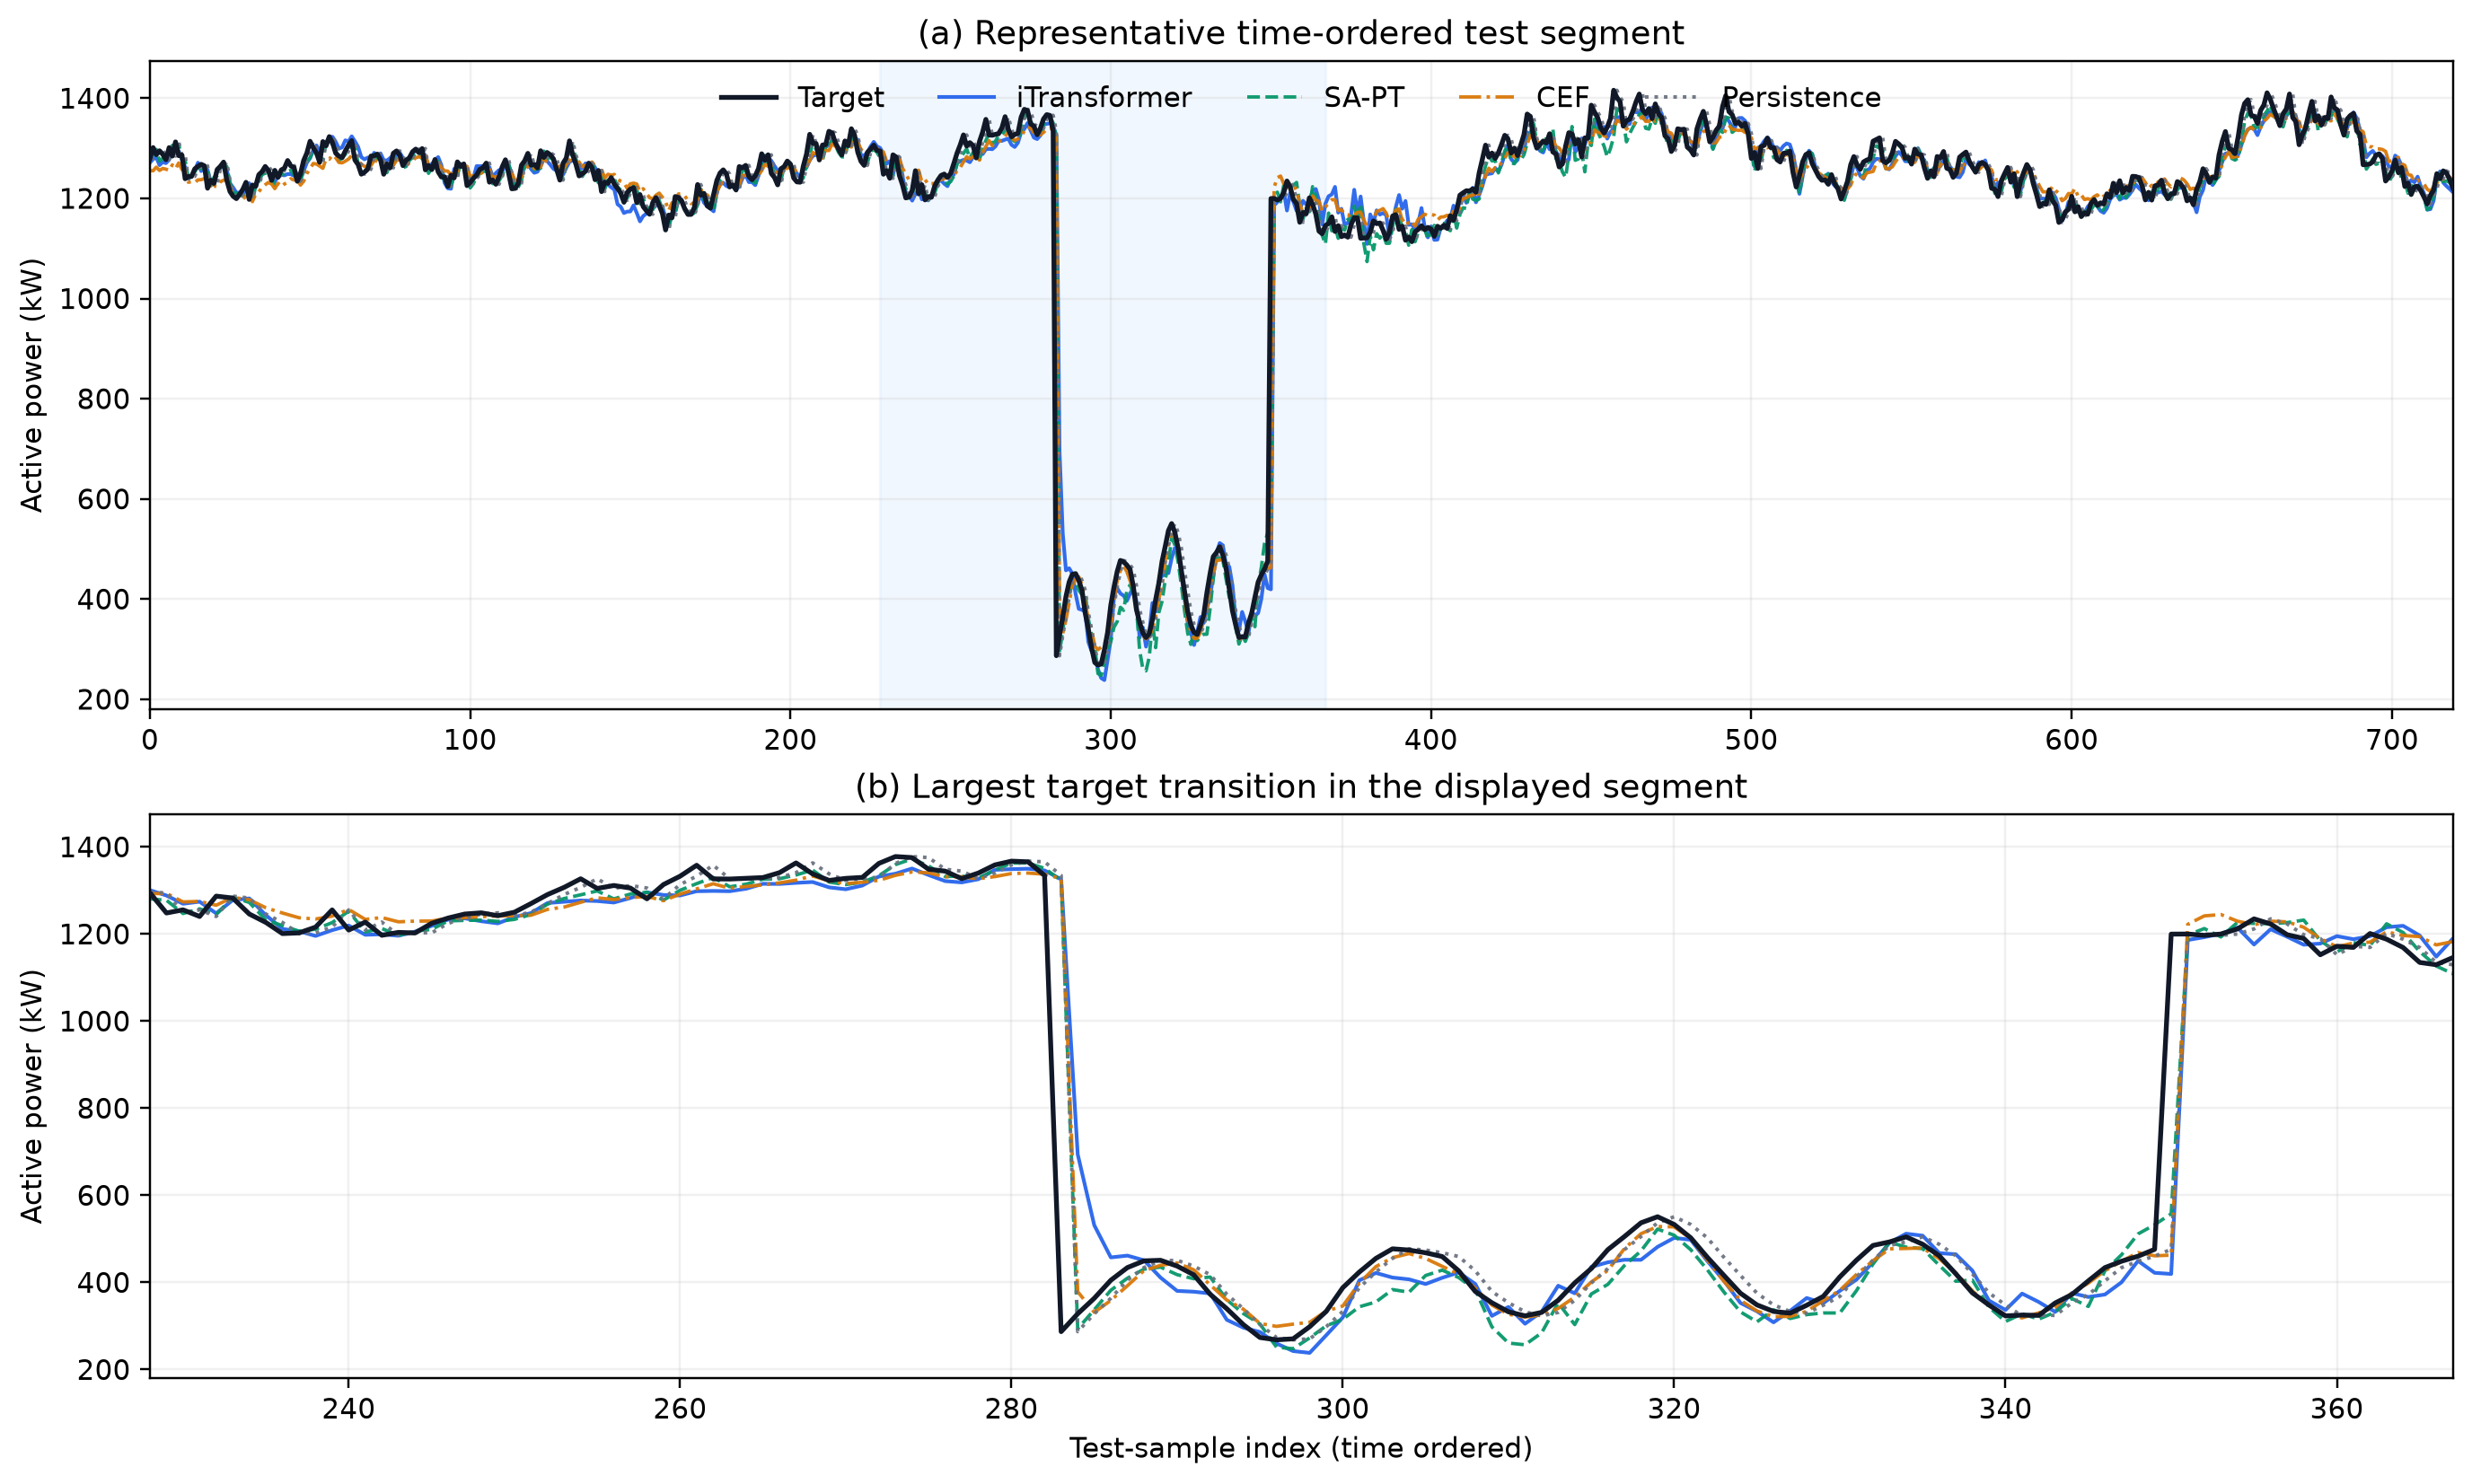
\includegraphics[width=\linewidth,keepaspectratio]{../figures/fig04_target_domain_forecast_traces_en.png}
\caption{Representative forecast traces and transition detail}
\label{fig:forecast-traces}
\end{figure}

\begin{figure}
\centering
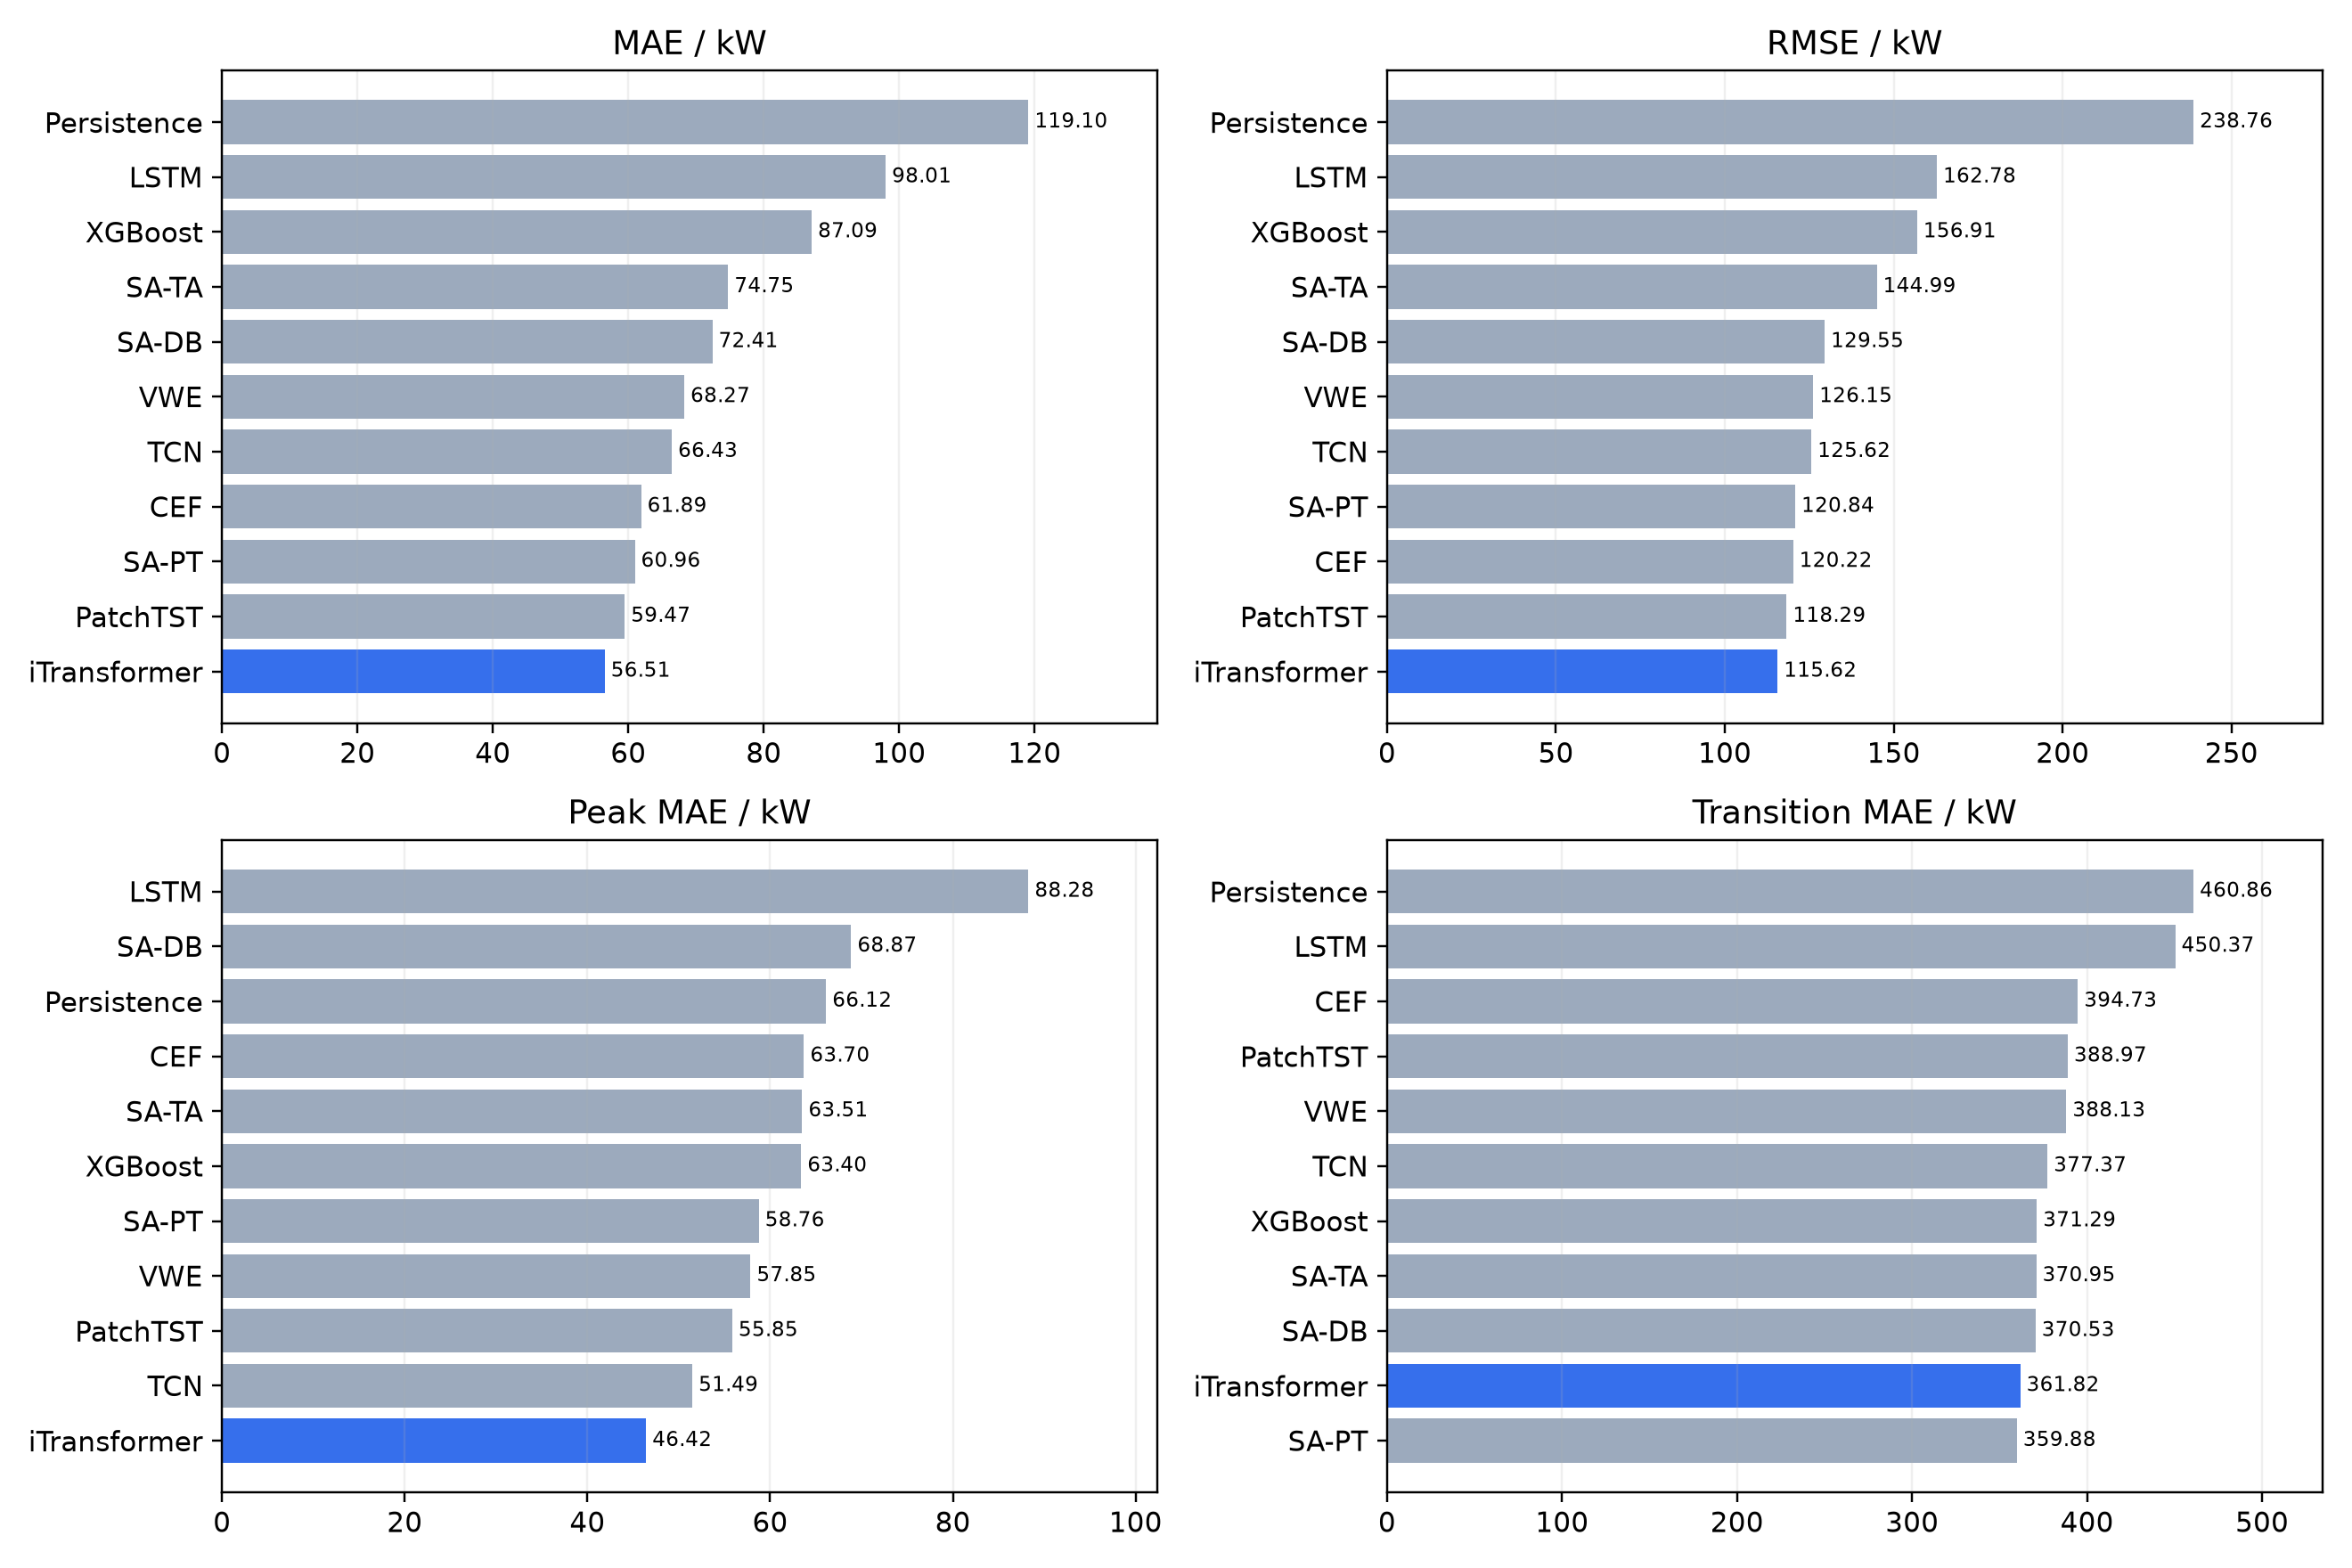
\includegraphics[width=\linewidth,keepaspectratio]{../figures/fig05_target_domain_forecast_metrics_en.png}
\caption{Forecast metric comparison for all candidates}
\label{fig:forecast-metrics}
\end{figure}

\begin{table}[!t]
\caption{Forecasting comparison on the evaluation replay}
\label{tab:forecast-comparison}
\centering
\footnotesize
\begin{tabular}{@{}
  >{\raggedright\arraybackslash}p{(\linewidth - 10\tabcolsep) * \real{0.2000}}
  >{\raggedleft\arraybackslash}p{(\linewidth - 10\tabcolsep) * \real{0.1600}}
  >{\raggedleft\arraybackslash}p{(\linewidth - 10\tabcolsep) * \real{0.1600}}
  >{\raggedleft\arraybackslash}p{(\linewidth - 10\tabcolsep) * \real{0.1600}}
  >{\raggedleft\arraybackslash}p{(\linewidth - 10\tabcolsep) * \real{0.1600}}
  >{\raggedleft\arraybackslash}p{(\linewidth - 10\tabcolsep) * \real{0.1600}}@{}}
\toprule
\begin{minipage}[b]{\linewidth}\raggedright
Model
\end{minipage} & \begin{minipage}[b]{\linewidth}\raggedleft
MAE (kW)
\end{minipage} & \begin{minipage}[b]{\linewidth}\raggedleft
RMSE (kW)
\end{minipage} & \begin{minipage}[b]{\linewidth}\raggedleft
$R^2$
\end{minipage} & \begin{minipage}[b]{\linewidth}\raggedleft
Peak MAE (kW)
\end{minipage} & \begin{minipage}[b]{\linewidth}\raggedleft
Transition MAE (kW)
\end{minipage} \\
\midrule
iTransformer & 56.51 & 115.62 & 0.94 & 46.42 & 361.82 \\
PatchTST & 59.47 & 118.30 & 0.94 & 55.85 & 388.97 \\
SA-PT & 60.96 & 120.84 & 0.93 & 58.76 &
359.88 \\
CEF & 61.89 & 120.22 & 0.93 & 63.70 &
394.73 \\
TCN & 66.43 & 125.62 & 0.93 & 51.49 & 377.38 \\
VWE & 68.27 & 126.15 & 0.93 & 57.85 &
388.13 \\
SA-DB & 72.41 & 129.55 & 0.92 &
68.87 & 370.53 \\
SA-TA & 74.75 & 144.99 & 0.90 & 63.51 &
370.95 \\
XGBoost & 87.09 & 156.91 & 0.89 & 63.40 & 371.29 \\
LSTM & 98.01 & 162.78 & 0.88 & 88.28 & 450.37 \\
Persistence & 119.10 & 238.76 & 0.74 & 66.13 & 460.86 \\
\bottomrule
\end{tabular}
\end{table}

\subsection{Ten-holdout dispatch
comparison}\label{frozen-dispatch-comparison}

Table~\ref{tab:aggregate-dispatch-results} reports aggregate results for all seven online controllers across ten
independently generated eligible holdouts. The prespecified primary
inferential contrasts in this subsection are RSS versus RB and MLR. SC and RAC
also serve as factorial arms in the mechanism analysis, whereas P-MPC and RAE
are retained as secondary descriptive comparators. RSS produces 813.43 kWh of
unserved energy, compared with 840.96 kWh for RB and 906.04 kWh for MLR,
corresponding to reductions of 3.27\% and 10.22\%, respectively. Its aggregate
risk-adjusted cost is 95,366.92 yuan, 3.85\% below RB and 9.34\% below MLR.

Risk-adjusted cost is not independent economic evidence. It includes the
declared 100 yuan/kWh unserved-energy penalty, which contributes approximately
85\% of the reported RSS, RB, and MLR totals. Consequently, the cost comparison
is mechanically coupled to the reliability comparison and is interpreted as a
composite monetary summary rather than a second independent outcome. RSS uses
37.20 L less diesel than RB but 2.61 L more than MLR; fuel use is therefore
reported separately from the composite cost.

The seed is the independent analysis unit; the three scenarios remain
clustered within each seed. RSS minus RB is $-2.75\pm5.39$ kWh (mean $\pm$
sample SD; seed-bootstrap 95\% interval, $-6.36$ to $-0.29$ kWh), and RSS
minus MLR is $-9.26\pm11.31$ kWh (interval, $-16.31$ to $-3.33$ kWh). RSS is
lower or tied on every seed: 7 improvements and 3 ties against RB, and 9
improvements and 1 tie against MLR. Exact two-sided sign-flip $p$-values are
0.02 and $<0.01$; the corresponding Holm-adjusted values are 0.02 and 0.01.
All 210 main online method--scenario trajectories pass the physical audit, and
the maximum RSS decision time is 0.36 s.

Figure~\ref{fig:dispatch-connection-transition} shows an illustrative dispatch and SOC trajectory during a
connection-transition replay. To retain legibility at manuscript size, it
displays the three prespecified main-comparison methods (RB, MLR, and RSS).
Table~\ref{tab:aggregate-dispatch-results} reports all seven online controllers; SC and RAC are revisited as
mechanism arms, while P-MPC and RAE remain descriptive comparators.

\begin{figure}
\centering
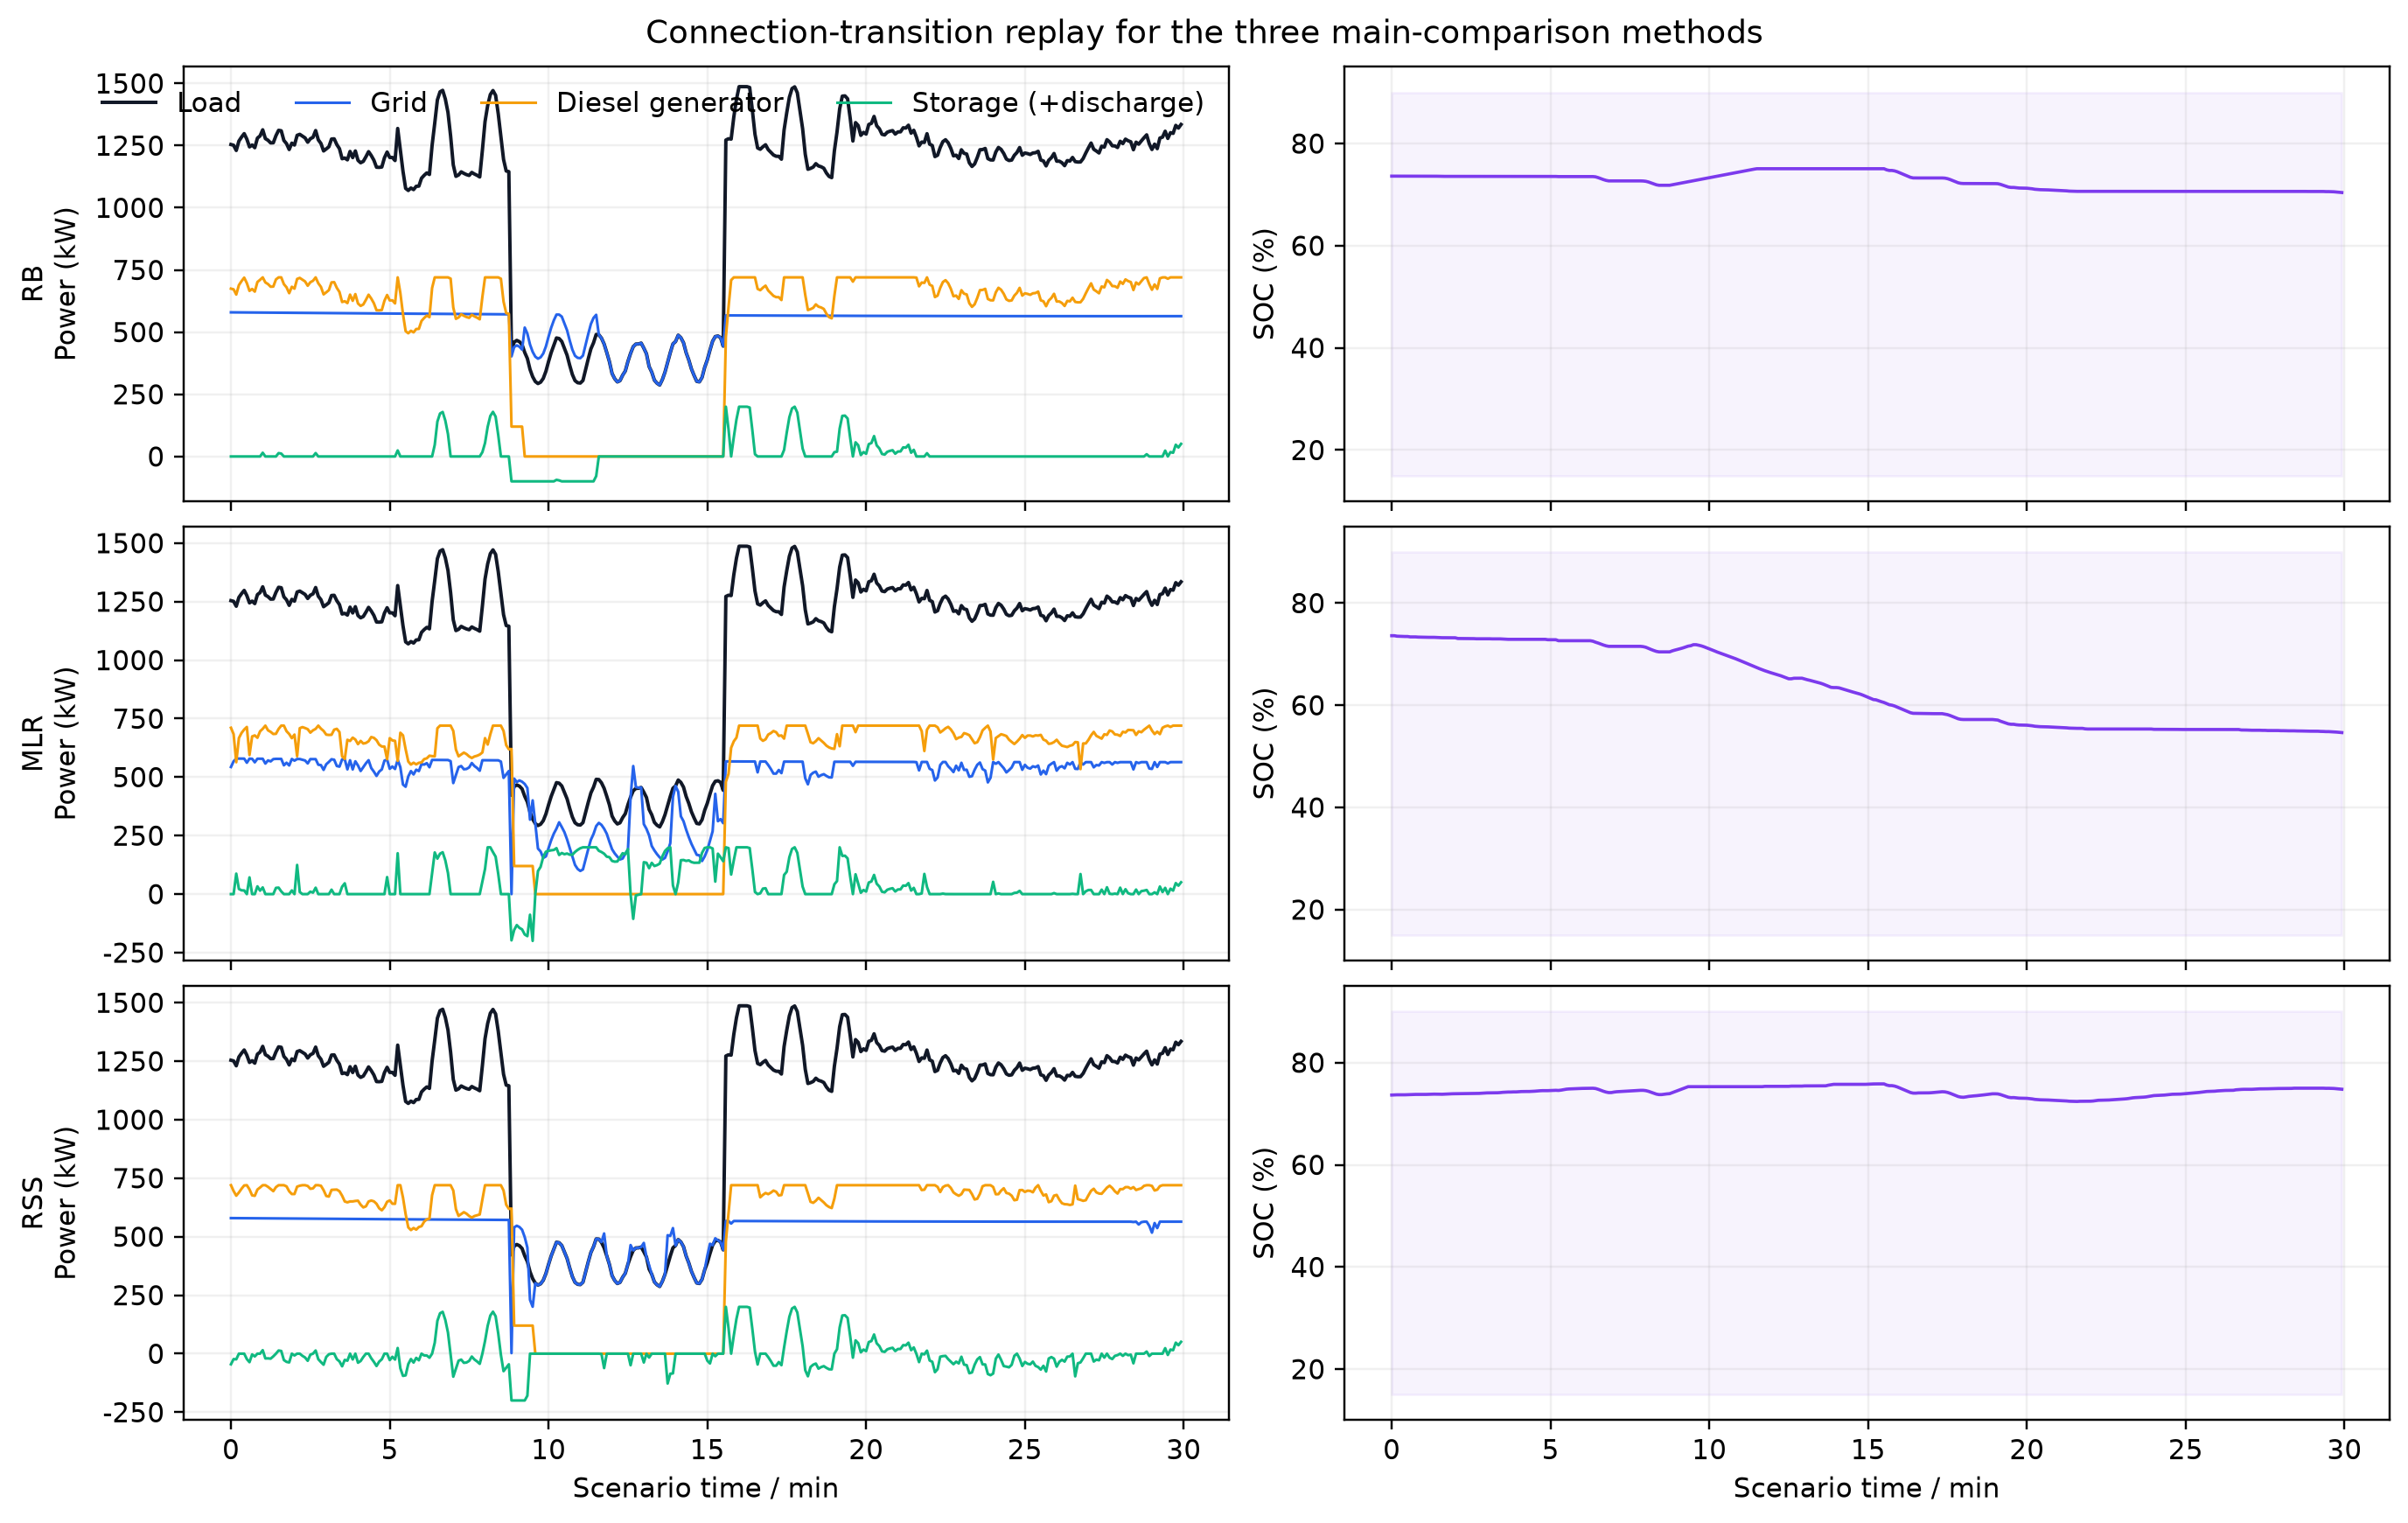
\includegraphics[width=\linewidth,keepaspectratio]{../figures/fig06_dispatch_connection_transition_en.png}
\caption{Dispatch and SOC behavior of RB, MLR, and RSS during a connection transition}
\label{fig:dispatch-connection-transition}
\end{figure}

\clearpage
\begin{table}[!t]
\caption{Aggregate ten-holdout dispatch results for all seven online controllers}
\label{tab:aggregate-dispatch-results}
\centering
\footnotesize
\begin{tabular}{@{}
  >{\raggedright\arraybackslash}p{(\linewidth - 8\tabcolsep) * \real{0.1579}}
  >{\raggedleft\arraybackslash}p{(\linewidth - 8\tabcolsep) * \real{0.2105}}
  >{\raggedleft\arraybackslash}p{(\linewidth - 8\tabcolsep) * \real{0.2105}}
  >{\raggedleft\arraybackslash}p{(\linewidth - 8\tabcolsep) * \real{0.2105}}
  >{\raggedleft\arraybackslash}p{(\linewidth - 8\tabcolsep) * \real{0.2105}}@{}}
\toprule
\begin{minipage}[b]{\linewidth}\raggedright
Method
\end{minipage} & \begin{minipage}[b]{\linewidth}\raggedleft
Unserved energy (kWh)
\end{minipage} & \begin{minipage}[b]{\linewidth}\raggedleft
Risk-adjusted cost (yuan)
\end{minipage} & \begin{minipage}[b]{\linewidth}\raggedleft
Diesel fuel (L)
\end{minipage} & \begin{minipage}[b]{\linewidth}\raggedleft
Maximum decision time (s)
\end{minipage} \\
\midrule
RSS & 813.43 & 95,366.92 & 722.32 & 0.36 \\
RB & 840.96 & 99,189.91 & 759.52 & 0.00 \\
MLR & 906.04 & 105,192.33 & 719.71 & 0.12 \\
P-MPC & 1,070.88 & 121,964.13 & 713.08 & 0.10 \\
SC & 842.01 & 98,411.06 & 703.01 & 0.40 \\
RAC & 854.49 & 99,621.09 & 696.11 & 0.40 \\
RAE & 844.79 & 98,847.86 & 719.06 & 0.12 \\
\bottomrule
\end{tabular}
\end{table}

Values displayed as 0.00 are nonnegative recorded times below half of the final
reporting unit.

The per-holdout descriptive table below is restricted to RSS, RB, and MLR
because it supports the two primary paired contrasts; Table~\ref{tab:aggregate-dispatch-results} is the complete
aggregate comparison of the seven online controllers.

Figure~\ref{fig:paired-controller-effects}(a) summarizes the seed-level controller contrasts for the ten
independent holdouts and preserves the seed as the analysis unit. Figure~\ref{fig:paired-controller-effects}(b)
reports mean paired mechanism effects with seed-bootstrap 95\% intervals. The
risk-on minus risk-off effect is exactly 0.00 kWh for every seed, so it is
shown explicitly as a zero-width interval rather than as an apparently empty
plot.

\begin{figure}
\centering
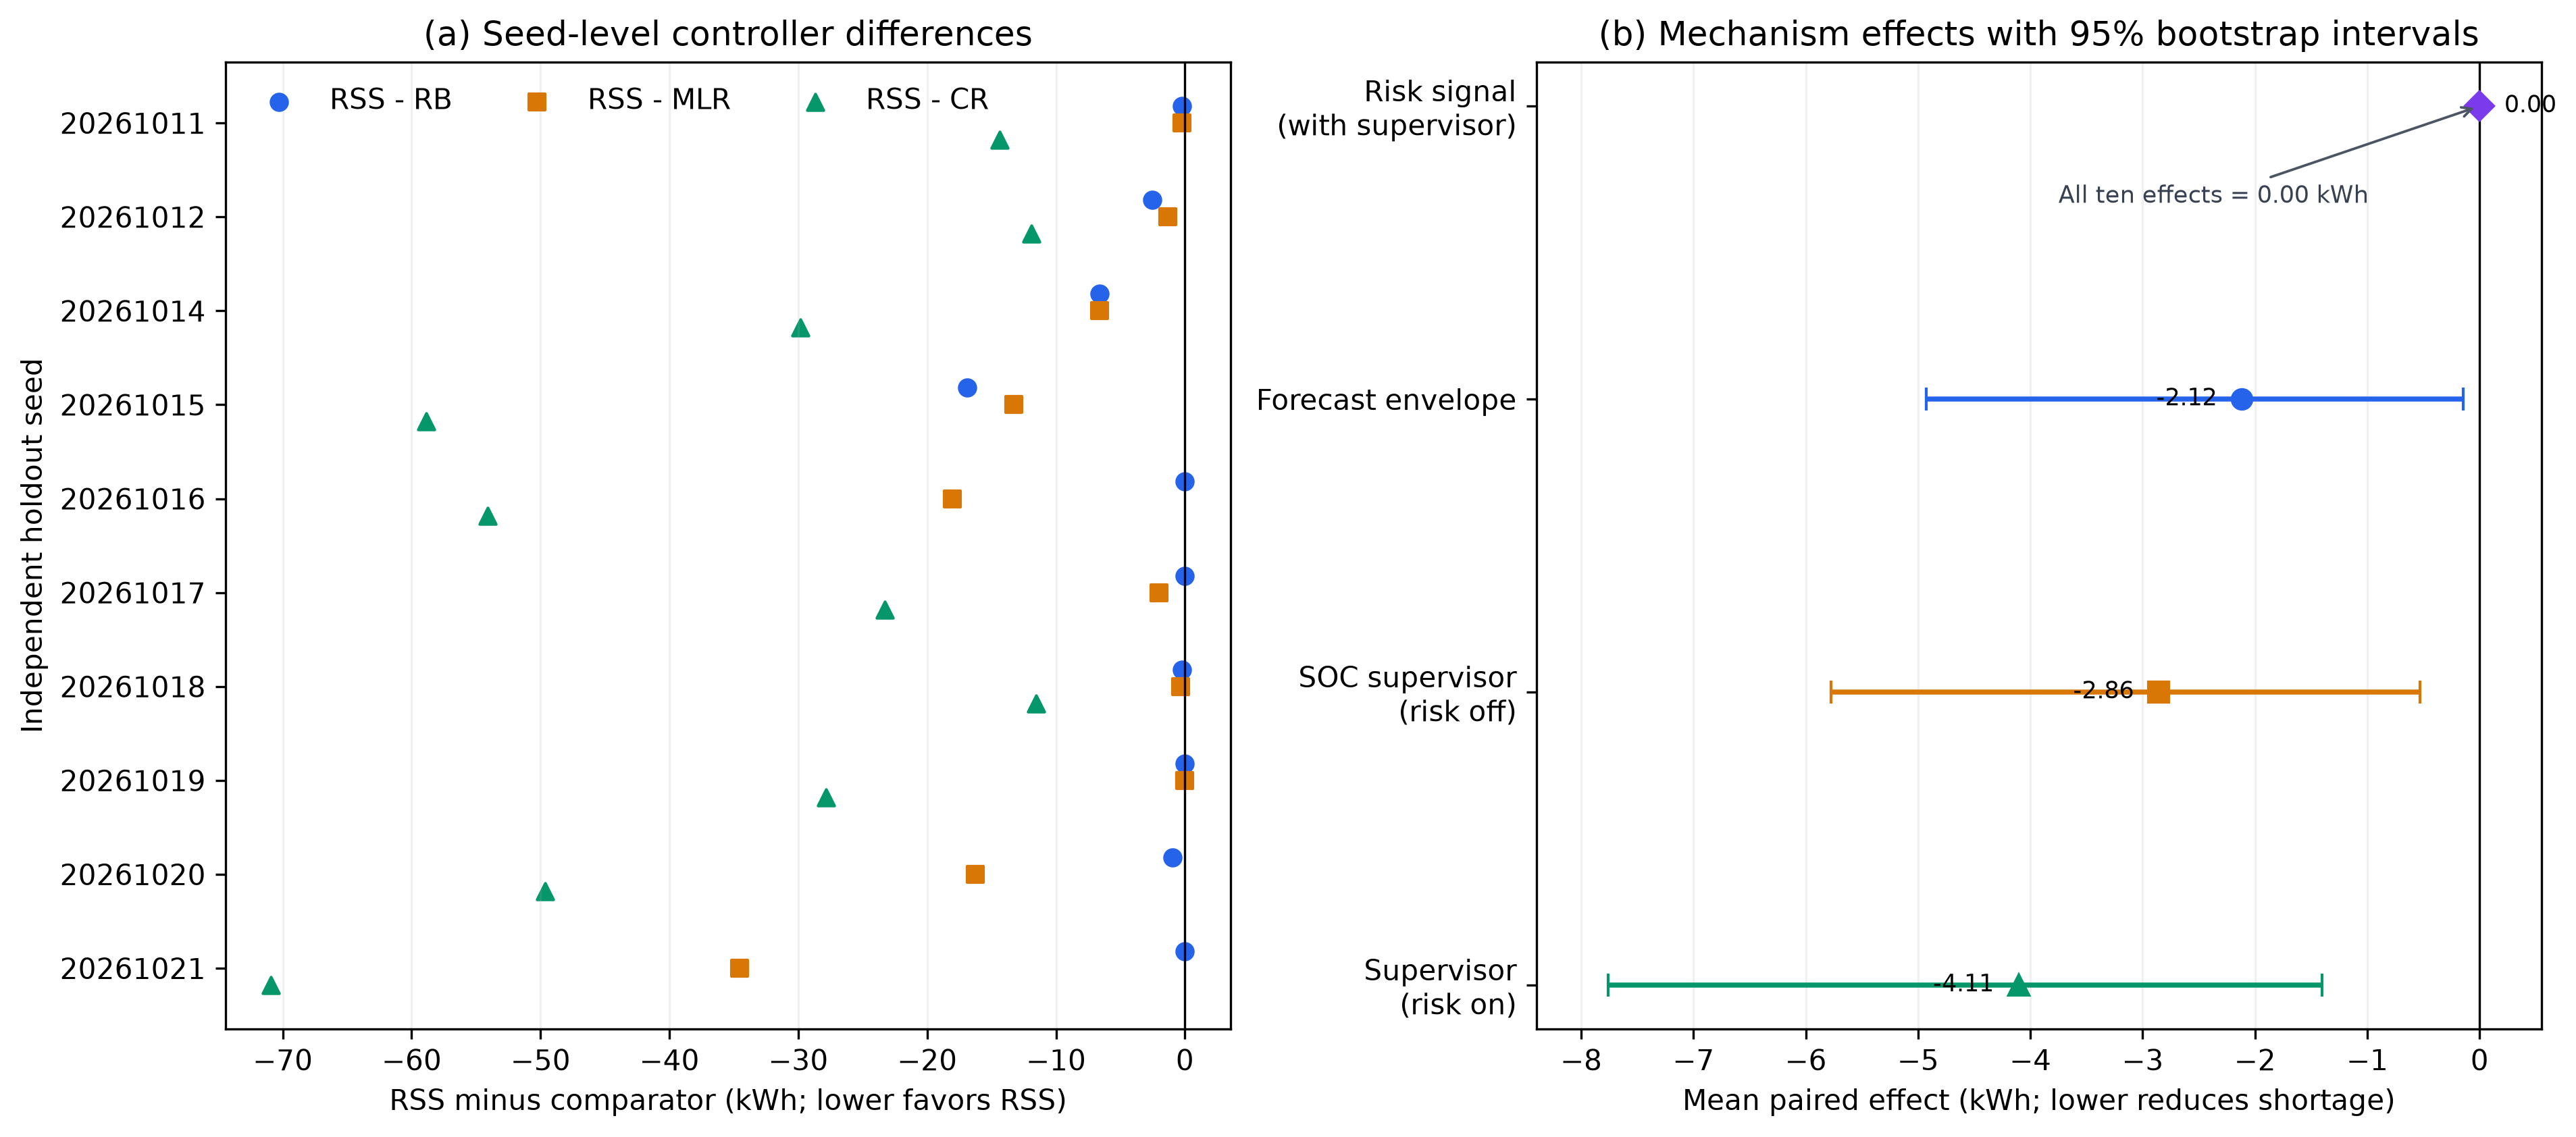
\includegraphics[width=\linewidth,keepaspectratio]{../experiments/results/extended_holdout_analysis.png}
\caption{Ten-holdout paired controller differences and mechanism effects}
\label{fig:paired-controller-effects}
\end{figure}

\clearpage
Table~\ref{tab:per-holdout-comparison} reports the per-holdout safety and descriptive comparison.

\begin{table}[!t]
\caption{Per-holdout safety and descriptive comparison}
\label{tab:per-holdout-comparison}
\centering
\scriptsize
\begin{tabular}{@{}
  >{\raggedleft\arraybackslash}p{(\linewidth - 12\tabcolsep) * \real{0.1481}}
  >{\raggedleft\arraybackslash}p{(\linewidth - 12\tabcolsep) * \real{0.1481}}
  >{\raggedleft\arraybackslash}p{(\linewidth - 12\tabcolsep) * \real{0.1481}}
  >{\raggedleft\arraybackslash}p{(\linewidth - 12\tabcolsep) * \real{0.1481}}
  >{\raggedleft\arraybackslash}p{(\linewidth - 12\tabcolsep) * \real{0.1481}}
  >{\raggedleft\arraybackslash}p{(\linewidth - 12\tabcolsep) * \real{0.1481}}
  >{\raggedright\arraybackslash}p{(\linewidth - 12\tabcolsep) * \real{0.1111}}@{}}
\toprule
\begin{minipage}[b]{\linewidth}\raggedleft
Seed
\end{minipage} & \begin{minipage}[b]{\linewidth}\raggedleft
RSS unserved (kWh)
\end{minipage} & \begin{minipage}[b]{\linewidth}\raggedleft
RB (kWh)
\end{minipage} & \begin{minipage}[b]{\linewidth}\raggedleft
MLR (kWh)
\end{minipage} & \begin{minipage}[b]{\linewidth}\raggedleft
Cost ratio
\end{minipage} & \begin{minipage}[b]{\linewidth}\raggedleft
Worst regret (kWh)
\end{minipage} & \begin{minipage}[b]{\linewidth}\raggedright
Audit
\end{minipage} \\
\midrule
20261011 & 104.56 & 104.81 & 104.78 & 0.99 & 0.00 & pass \\
20261012 & 104.49 & 107.03 & 105.82 & 0.99 & 0.00 & pass \\
20261014 & 138.81 & 145.45 & 145.45 & 0.96 & 0.00 & pass \\
20261015 & 159.24 & 176.15 & 172.50 & 0.93 & 0.00 & pass \\
20261016 & 65.19 & 65.23 & 83.23 & 0.81 & 0.00 & pass \\
20261017 & 5.48 & 5.48 & 7.48 & 0.88 & 0.00 & pass \\
20261018 & 71.97 & 72.18 & 72.31 & 0.97 & 0.00 & pass \\
20261019 & 9.03 & 9.03 & 9.03 & 0.96 & 0.00 & pass \\
20261020 & 134.97 & 135.92 & 151.23 & 0.90 & 0.00 & pass \\
20261021 & 19.68 & 19.68 & 54.22 & 0.49 & 0.00 & pass \\
\bottomrule
\end{tabular}
\end{table}

The cost ratio is RSS risk-adjusted cost divided by MLR risk-adjusted cost
for the same holdout seed.

\subsection{Independent causal full-MILP comparator and perfect-foresight reference}
\label{independent-full-milp-oracle-reference}

The causal rolling full-MILP reference (CR) is implemented independently from
the proposed controller. At each 5 s decision point, it solves a 12-step unit-
commitment and storage problem and applies the first action. CR uses the same
realized plant state, current capacity measurements, CEF point forecast, and
cost terms as RSS. It includes integer commitment, minimum stable output,
ramping, minimum up/down time, startup and shutdown logic, storage dynamics,
and mutually exclusive charging and discharging, but excludes the forecast-
error envelope and reserve--SOC supervisor.

CR and RSS share the post-warm-up SOC, generator outputs, committed-unit count,
and binding startup and shutdown history. Unit tests verify the minimum up/down
constraints at the comparison boundary.

Across ten holdouts, CR produces 1,165.81 kWh of unserved energy, compared with
813.43 kWh for RSS, a reduction of 30.23\%. RSS minus CR is
$-35.24\pm21.50$ kWh at the seed level (seed-bootstrap 95\% interval,
$-48.04$ to $-22.95$ kWh); all ten differences favor RSS. The exact two-sided
sign-flip $p$-value is $<0.01$ and its Holm-adjusted value is 0.01. Mean CR solve
time is 0.01 s per decision and the maximum is 0.19 s. All 30 trajectories have
zero recorded power-balance residual and charge--discharge product.

CR also produces more unserved energy than RB, which records 840.96 kWh in
Table~\ref{tab:aggregate-dispatch-results}. The controller definitions provide a plausible explanation framework
but do not identify the cause of this ordering. CR optimizes a 12-step causal
point forecast and has neither the forecast envelope nor the reserve--SOC
supervisor; it therefore lacks both explicit forecast-dispersion coverage and
the SOC-triggered reserve preparation used by RSS. These differences are
sufficient to show that CR is not a like-for-like component ablation. They are
not sufficient to attribute the CR--RB gap to a particular mechanism: the
available RSS-centered interventions do not decompose CR against RB one change
at a time. We therefore treat CR as a bundled causal boundary comparator and do
not infer that full-MILP control is intrinsically worse than rule-based control
or that either omitted component alone explains the observed gap.

The perfect-foresight reference (PF) solves the same 30 min dispatch problem
with the realized load trajectory available over the full horizon. It includes
the generator, storage, dynamic-capacity, and cost constraints used in the
online comparison, retains a terminal SOC reserve of $5.00\times10^{-3}$, and
uses a linear rated-point fuel approximation. PF minimizes the composite
operating objective and provides a best-case reference for the original two
holdouts.

On the original two holdouts, PF produces 201.83 kWh of total unserved energy
versus 209.05 kWh for RSS. The two PF totals are 82.84 and 118.99 kWh, with
optimal solver status for all six scenario windows. The maximum
power-balance residual is $2.30\times10^{-13}$ kW, the maximum
charge--discharge product is zero, and the mean solve time is 0.26 s per
scenario window.

Scopes differ and are shown explicitly in Table~\ref{tab:full-milp-references}; RSS is included for context.

\begin{table}[!t]
\caption{Independent causal and perfect-foresight full-MILP references.}
\label{tab:full-milp-references}
\centering
\footnotesize
\begin{tabular}{>{\raggedright\arraybackslash}p{4.6cm}r >{\raggedright\arraybackslash}p{5.0cm}}
\toprule
Reference and scope & Unserved (kWh) & Solve time / audit \\
\midrule
RSS, ten holdouts & 813.43 & causal scenario/supervisory pipeline; max 0.36 s/decision; pass \\
CR, ten holdouts & 1,165.81 & causal 12-step point forecast; mean 0.01, max 0.19 s/decision; pass \\
PF, original two holdouts & 201.83 & realized 30-min load; mean 0.26 s/window; pass \\
\bottomrule
\end{tabular}
\end{table}

\subsection{Orthogonal risk-by-supervisor mechanism
audit}\label{mechanism-ablation-from-frozen-holdout-rows}

The mechanism audit forms a 2$\times$2 design on the same ten seeds, scenario
windows, plant, forecast envelope, costs, and solver settings. SC has static
scenario CVaR without adaptive risk or the supervisor; RAC adds adaptive risk
without the supervisor; RSS-R0 activates the reserve--SOC supervisor while
neutralizing only the predicted/dispatch risk level and reserve adder; and RSS
activates both. The risk-off intervention holds the SOC thresholds,
hysteresis, generator-first reserve logic, grid-headroom rule, capacity traces,
and shared warm-up fixed. The 30 newly generated RSS-R0 method--scenario
trajectories pass the physical audit; the SC, RAC, and RSS arms reuse the
corresponding main-comparison trajectories covered by the main audit.

Within the specified SC/RAC-centered intervention, activating the supervisor is
associated with a change in mean seed-level unserved energy
by $-2.86$ kWh (RSS-R0 minus SC); with adaptive risk, its change is $-4.11$ kWh
(RSS minus RAC). Neither effect is adverse on any seed; exact two-sided
sign-flip $p$-values are 0.03 and 0.02. Adaptive risk without the supervisor
changes the mean by $+1.25$ kWh (RAC minus SC), while the clean marginal risk
contrast under the supervisor is 0.00 kWh on every seed. The aggregate
risk-adjusted-cost difference between risk-on and risk-off supervision is
$-15.23$ yuan, while shortage is identical to numerical precision.

The trace-level overlap audit is consistent with the null shortage effect.
Across 10,800 control steps, high risk occurs on 29.19\%, the risk channel
changes the internal protection mode on 8.78\%, and physical actions differ on
1.72\%. Under the implemented controller, the constrained optimizer and
reserve--SOC rules absorb most risk-level changes before they reach physical
actions. These intervention effects are local to the specified controller
configurations and do not constitute an additive decomposition of the
RSS--baseline differences.

Figure~\ref{fig:risk-action-overlap} visualizes why the marginal risk effect is negligible; Table~\ref{tab:risk-supervisor-audit}
reports the corresponding factorial arms.

\begin{figure}
\centering
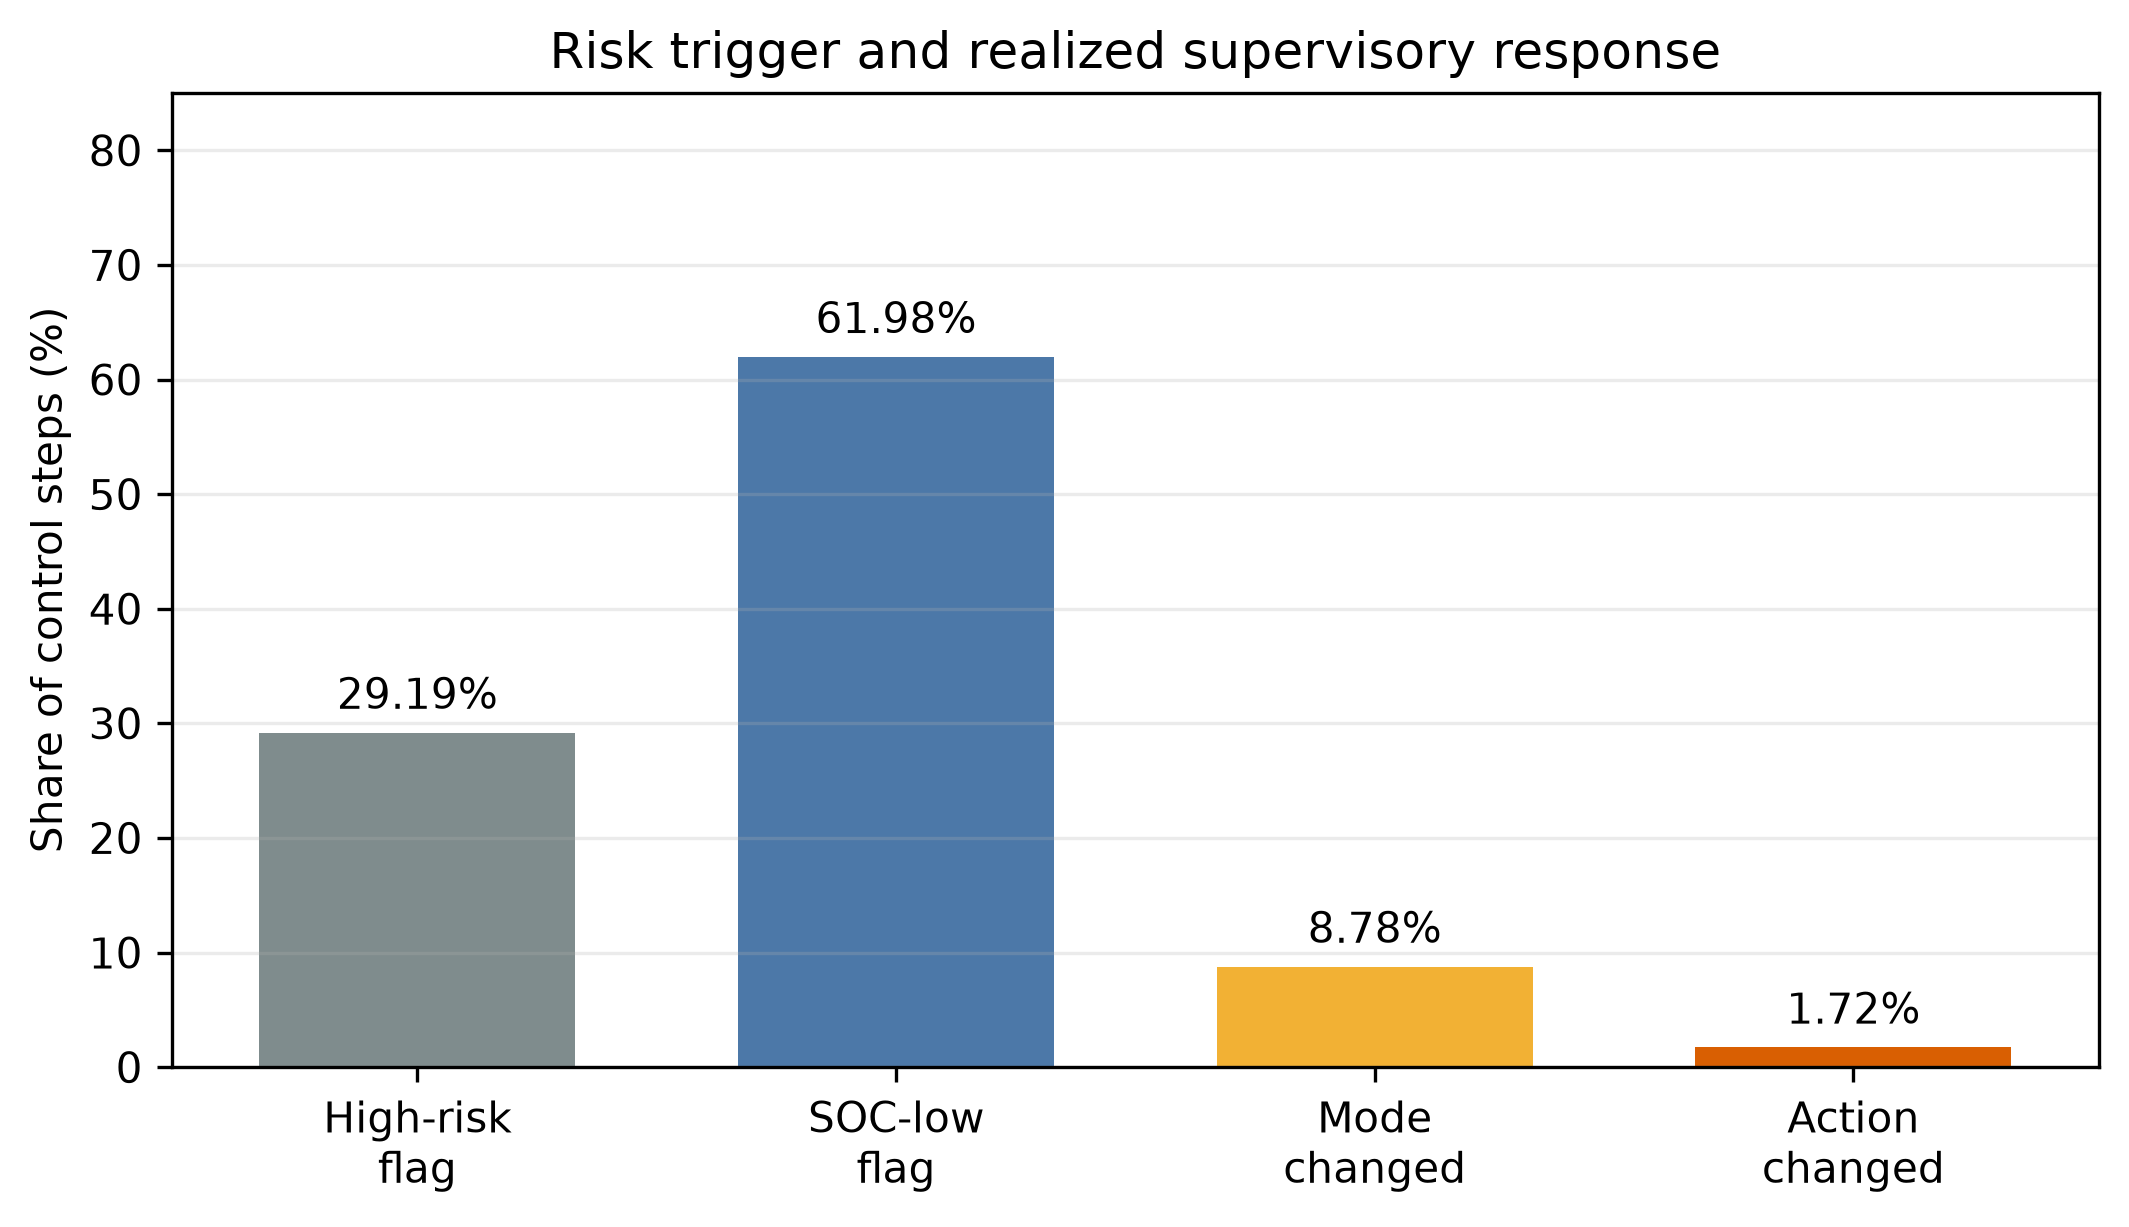
\includegraphics[width=0.82\linewidth,keepaspectratio]{../experiments/results/risk_action_overlap.png}
\caption{Risk trigger frequency and realized supervisory response}
\label{fig:risk-action-overlap}
\end{figure}

\begin{table}[!t]
\caption{Orthogonal risk-by-supervisor mechanism audit over ten holdouts.}
\label{tab:risk-supervisor-audit}
\centering
\footnotesize
\setlength{\tabcolsep}{4pt}
\begin{tabular}{lccrrr}
\toprule
Arm & Risk & Sup. & Unserved (kWh) & Cost (yuan) & Time (s) \\
\midrule
SC & off & off & 842.01 & 98,411.06 & 0.40 \\
RAC & on & off & 854.49 & 99,621.09 & 0.40 \\
RSS-R0 & off & on & 813.43 & 95,382.15 & 0.39 \\
RSS & on & on & 813.43 & 95,366.92 & 0.36 \\
\bottomrule
\end{tabular}
\end{table}

\subsection{Forecast uncertainty-envelope
ablation}\label{forecast-uncertainty-envelope-ablation}

The paired intervention tests the implemented forecast-envelope bundle over all
ten holdouts. It retains the risk signal, SOC supervisor, generator-first
execution, and physical constraints, while setting the fixed-reserve and
forecast-disagreement terms to zero and replacing all scenario members with the
same causal point forecast.

Within this paired RSS-centered intervention, the no-envelope variant increases
aggregate unserved energy from 813.43 to 834.61 kWh and risk-adjusted cost from
95,366.92 to 97,406.90 yuan, while reducing diesel use from 722.32 to 692.62 L.
The paired shortage difference (envelope on minus off) is $-2.12\pm4.34$ kWh
per seed, with a seed-bootstrap 95\% interval of $-4.93$ to $-0.15$ kWh and
exact two-sided sign-flip $p=0.03$. Six seeds improve and four tie; none worsens.
The registered no-envelope audit covers all 210 method--scenario trajectories
and 75,600 rows generated by the full online-controller rerun, whereas the
mechanism estimate uses only the paired RSS and RSS-NE outcomes. Within this
contrast, enabling the envelope bundle trades additional diesel use for lower
shortage and risk-adjusted cost; this local effect does not decompose the full
RSS--baseline differences. The no-envelope variant is denoted RSS-NE in
Table~\ref{tab:uncertainty-envelope-intervention}.

\begin{table}[!t]
\caption{Ten-holdout uncertainty-envelope intervention.}
\label{tab:uncertainty-envelope-intervention}
\centering
\footnotesize
\begin{tabular}{lrrrrc}
\toprule
Variant & Unserved (kWh) & Risk cost (yuan) & Diesel (L) & Max time (s) & Audit \\
\midrule
RSS & 813.43 & 95,366.92 & 722.32 & 0.36 & pass \\
RSS-NE & 834.61 & 97,406.90 & 692.62 & 0.32 & pass \\
\bottomrule
\end{tabular}
\end{table}

\subsection{Auxiliary risk-interface
diagnostics}\label{auxiliary-risk-interface-diagnostics}

The original risk classifier obtains Macro-F1 0.49, high-risk recall 0.78, and
severe-risk recall 0.85 on the forecasting replay. Neutralizing this signal in
the ten primary holdouts changes aggregate unserved energy by 0.00 kWh, showing
no marginal shortage effect for the risk signal in this intervention. This
result does not identify the sources of the primary RSS--baseline differences
or provide a complete mechanism decomposition.

The auxiliary E-RSS interface is evaluated on a separate six-holdout group. It
raises dispatch Macro-F1 from 0.73 to 0.76 and balanced accuracy from 0.75 to
0.79, while increasing the Brier score from 0.05 to 0.11. E-RSS changes 53 of
6,480 physical control rows, but aggregate unserved energy remains 335.23 kWh
for both variants and risk-adjusted cost changes from 42,420.31 to 42,419.01
yuan. The interface therefore improves Macro-F1 and balanced accuracy in this
group while worsening the Brier score; it exposes source conflict without
improving the primary energy-system outcomes.

A separate second six-holdout group evaluates Dempster combination and
temperature calibration. DC-RSS reduces mean Brier score from 0.07 for raw
D-RSS to 0.03 and raises Macro-F1 from 0.75 for RSS to 0.77. Calibration does
not change the selected risk class or dispatch action. Aggregate unserved energy
remains 466.05 kWh, and the 4.71 yuan cost difference is negligible relative to
the total risk-adjusted cost. Table~\ref{tab:risk-interface-diagnostics}
summarizes the diagnostic variants from this second holdout group. These results
support reporting classification and calibration effects separately from
dispatch outcomes; they do not provide evidence that the interface caused the
primary dispatch improvement reported in Section~\ref{frozen-dispatch-comparison}.

\begin{table}[!t]
\caption{Auxiliary conflict-rule and probability-calibration diagnostic on the
second six-holdout group.}
\label{tab:risk-interface-diagnostics}
\centering
\footnotesize
\begin{tabular}{@{}
  >{\raggedright\arraybackslash}p{(\linewidth - 10\tabcolsep) * \real{0.1429}}
  >{\raggedright\arraybackslash}p{(\linewidth - 10\tabcolsep) * \real{0.2857}}
  >{\raggedleft\arraybackslash}p{(\linewidth - 10\tabcolsep) * \real{0.1429}}
  >{\raggedleft\arraybackslash}p{(\linewidth - 10\tabcolsep) * \real{0.1429}}
  >{\raggedleft\arraybackslash}p{(\linewidth - 10\tabcolsep) * \real{0.1429}}
  >{\raggedleft\arraybackslash}p{(\linewidth - 10\tabcolsep) * \real{0.1429}}@{}}
\toprule
\begin{minipage}[b]{\linewidth}\raggedright
Variant
\end{minipage} & \begin{minipage}[b]{\linewidth}\raggedright
Probability layer
\end{minipage} & \begin{minipage}[b]{\linewidth}\raggedleft
Brier
\end{minipage} & \begin{minipage}[b]{\linewidth}\raggedleft
Macro-F1
\end{minipage} & \begin{minipage}[b]{\linewidth}\raggedleft
Changed actions vs RSS
\end{minipage} & \begin{minipage}[b]{\linewidth}\raggedleft
Unserved (kWh)
\end{minipage} \\
\midrule
RSS & learned output & 0.03 & 0.75 & 0 & 466.05 \\
E-RSS & raw Yager & 0.10 & 0.77 & 66 & 466.05 \\
D-RSS & raw Dempster & 0.07 & 0.77 & 57 & 466.05 \\
DC-RSS & Dempster, $T=0.50$ & 0.03 & 0.77 & 57 & 466.05 \\
\bottomrule
\end{tabular}
\end{table}

DC-RSS calibration changes the reported probability vector; its action and
control columns are shared with raw D-RSS.

\subsection{Emergency priority-load
ablation}\label{emergency-priority-load-ablation}

The emergency allocation diagnostic separates protection priority from
total supply adequacy. It compares proportional curtailment with a
priority-greedy allocator under the same stress scenarios.
The two policies produce the same total unserved energy in every
scenario, while priority protection transfers shortage away from
critical loads toward essential and interruptible loads. In the base
case, critical-load unserved energy decreases from 219.45 to 11.29
kWh; under the joint extreme stress, it decreases from 1,034.90 to
231.16 kWh. The corresponding total unserved energy remains 366.22 and
1,679.26 kWh, respectively.

Load prioritization changes the distribution of shortage, not the amount of
available supply. The class fractions used here are control-study settings
that require site-specific electrical and safety approval before deployment.

Figure~\ref{fig:emergency-priority-ablation} shows the critical-load and total-shortage comparison across the five
stress scenarios; Table~\ref{tab:emergency-priority-ablation} reports the corresponding values.

\begin{figure}
\centering
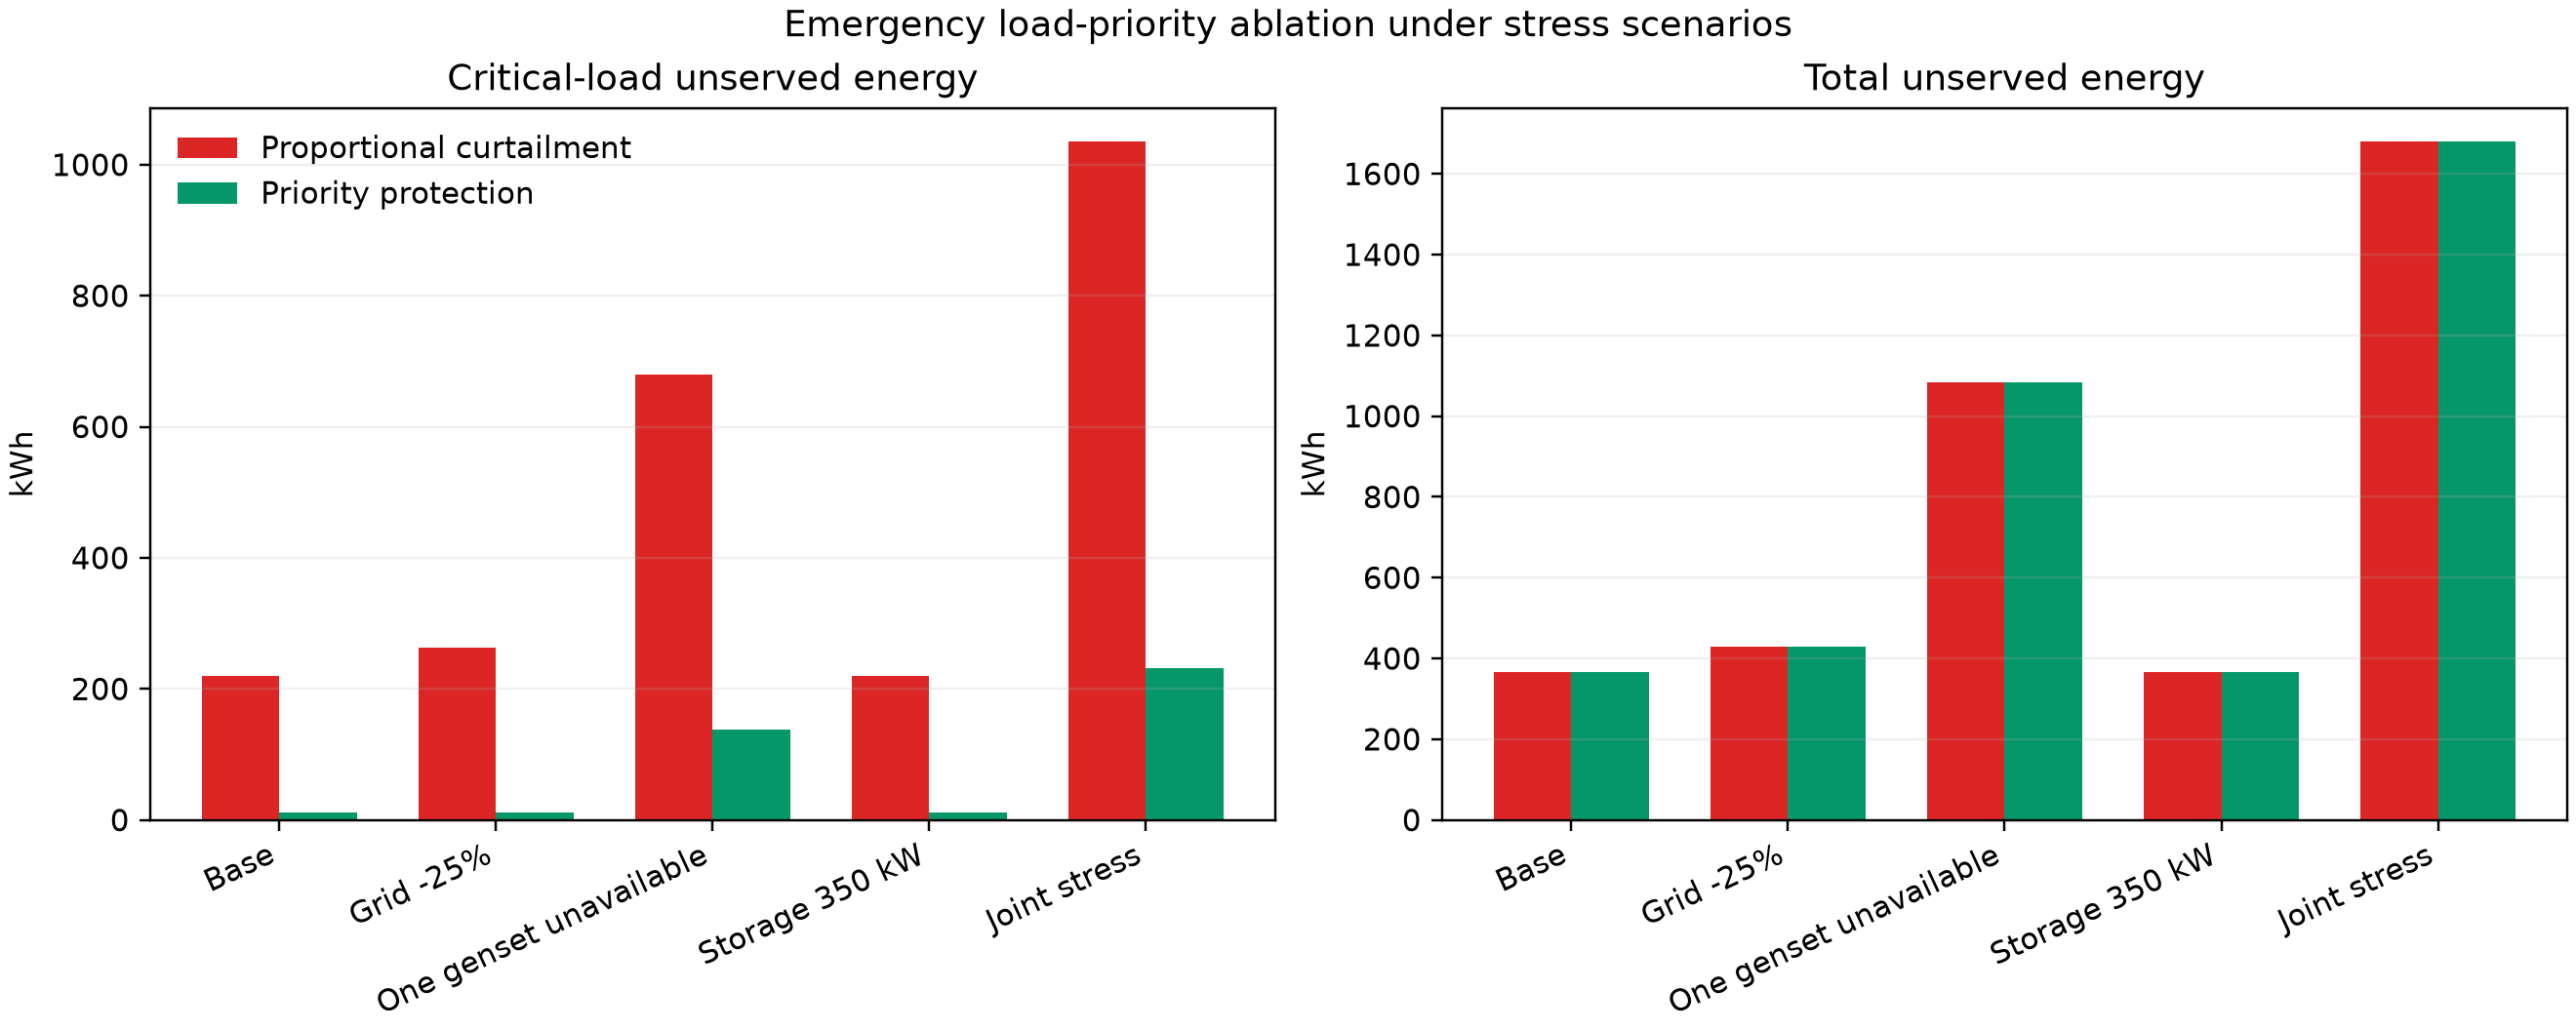
\includegraphics[width=\linewidth,keepaspectratio]{../experiments/results/emergency_priority_ablation/emergency_priority_ablation.png}
\caption{Emergency load-priority ablation}
\label{fig:emergency-priority-ablation}
\end{figure}

\begin{table}[!t]
\caption{Emergency load priority ablation under stress scenarios.}
\label{tab:emergency-priority-ablation}
\centering
\footnotesize
\begin{tabular}{@{}
  >{\raggedright\arraybackslash}p{(\linewidth - 8\tabcolsep) * \real{0.1579}}
  >{\raggedleft\arraybackslash}p{(\linewidth - 8\tabcolsep) * \real{0.2105}}
  >{\raggedleft\arraybackslash}p{(\linewidth - 8\tabcolsep) * \real{0.2105}}
  >{\raggedleft\arraybackslash}p{(\linewidth - 8\tabcolsep) * \real{0.2105}}
  >{\raggedleft\arraybackslash}p{(\linewidth - 8\tabcolsep) * \real{0.2105}}@{}}
\toprule
\begin{minipage}[b]{\linewidth}\raggedright
Scenario
\end{minipage} & \begin{minipage}[b]{\linewidth}\raggedleft
Critical unserved: proportional (kWh)
\end{minipage} & \begin{minipage}[b]{\linewidth}\raggedleft
Critical unserved: priority (kWh)
\end{minipage} & \begin{minipage}[b]{\linewidth}\raggedleft
Reduction (kWh)
\end{minipage} & \begin{minipage}[b]{\linewidth}\raggedleft
Total unserved (kWh)
\end{minipage} \\
\midrule
Base & 219.45 & 11.29 & 208.16 & 366.22 \\
Grid derating, 25\% & 263.57 & 11.29 & 252.28 & 430.10 \\
One generator unavailable & 679.87 & 137.84 & 542.03 & 1,083.29 \\
Storage power cap, 350 kW & 219.45 & 11.29 & 208.16 & 366.22 \\
Joint extreme stress & 1,034.90 & 231.16 & 803.75 & 1,679.26 \\
\bottomrule
\end{tabular}
\end{table}

\subsection{Missing-data and combined-stress
diagnostics}\label{missing-data-and-combined-stress-diagnostics}

The missing-data diagnostic increases MAE from 83.94 kW without injected
missingness to 84.33 kW under the moderate condition and 90.66 kW under the
severe condition.

Under a combined disturbance involving 25\% grid derating, one unavailable
generator, a 350 kW storage power cap, a 10 percentage-point SOC bias, a
2.50\% load increase, and a 15 s telemetry delay, priority protection reduces
critical-load unserved energy from 1,034.90 to 231.16 kWh. Total unserved
energy remains 1,679.26 kWh because the allocation layer cannot increase
available supply.

Figure~\ref{fig:joint-stress-protection} shows the detailed joint-extreme trajectory, complementing the
cross-scenario comparison in Figure~\ref{fig:emergency-priority-ablation}.

\begin{figure}
\centering
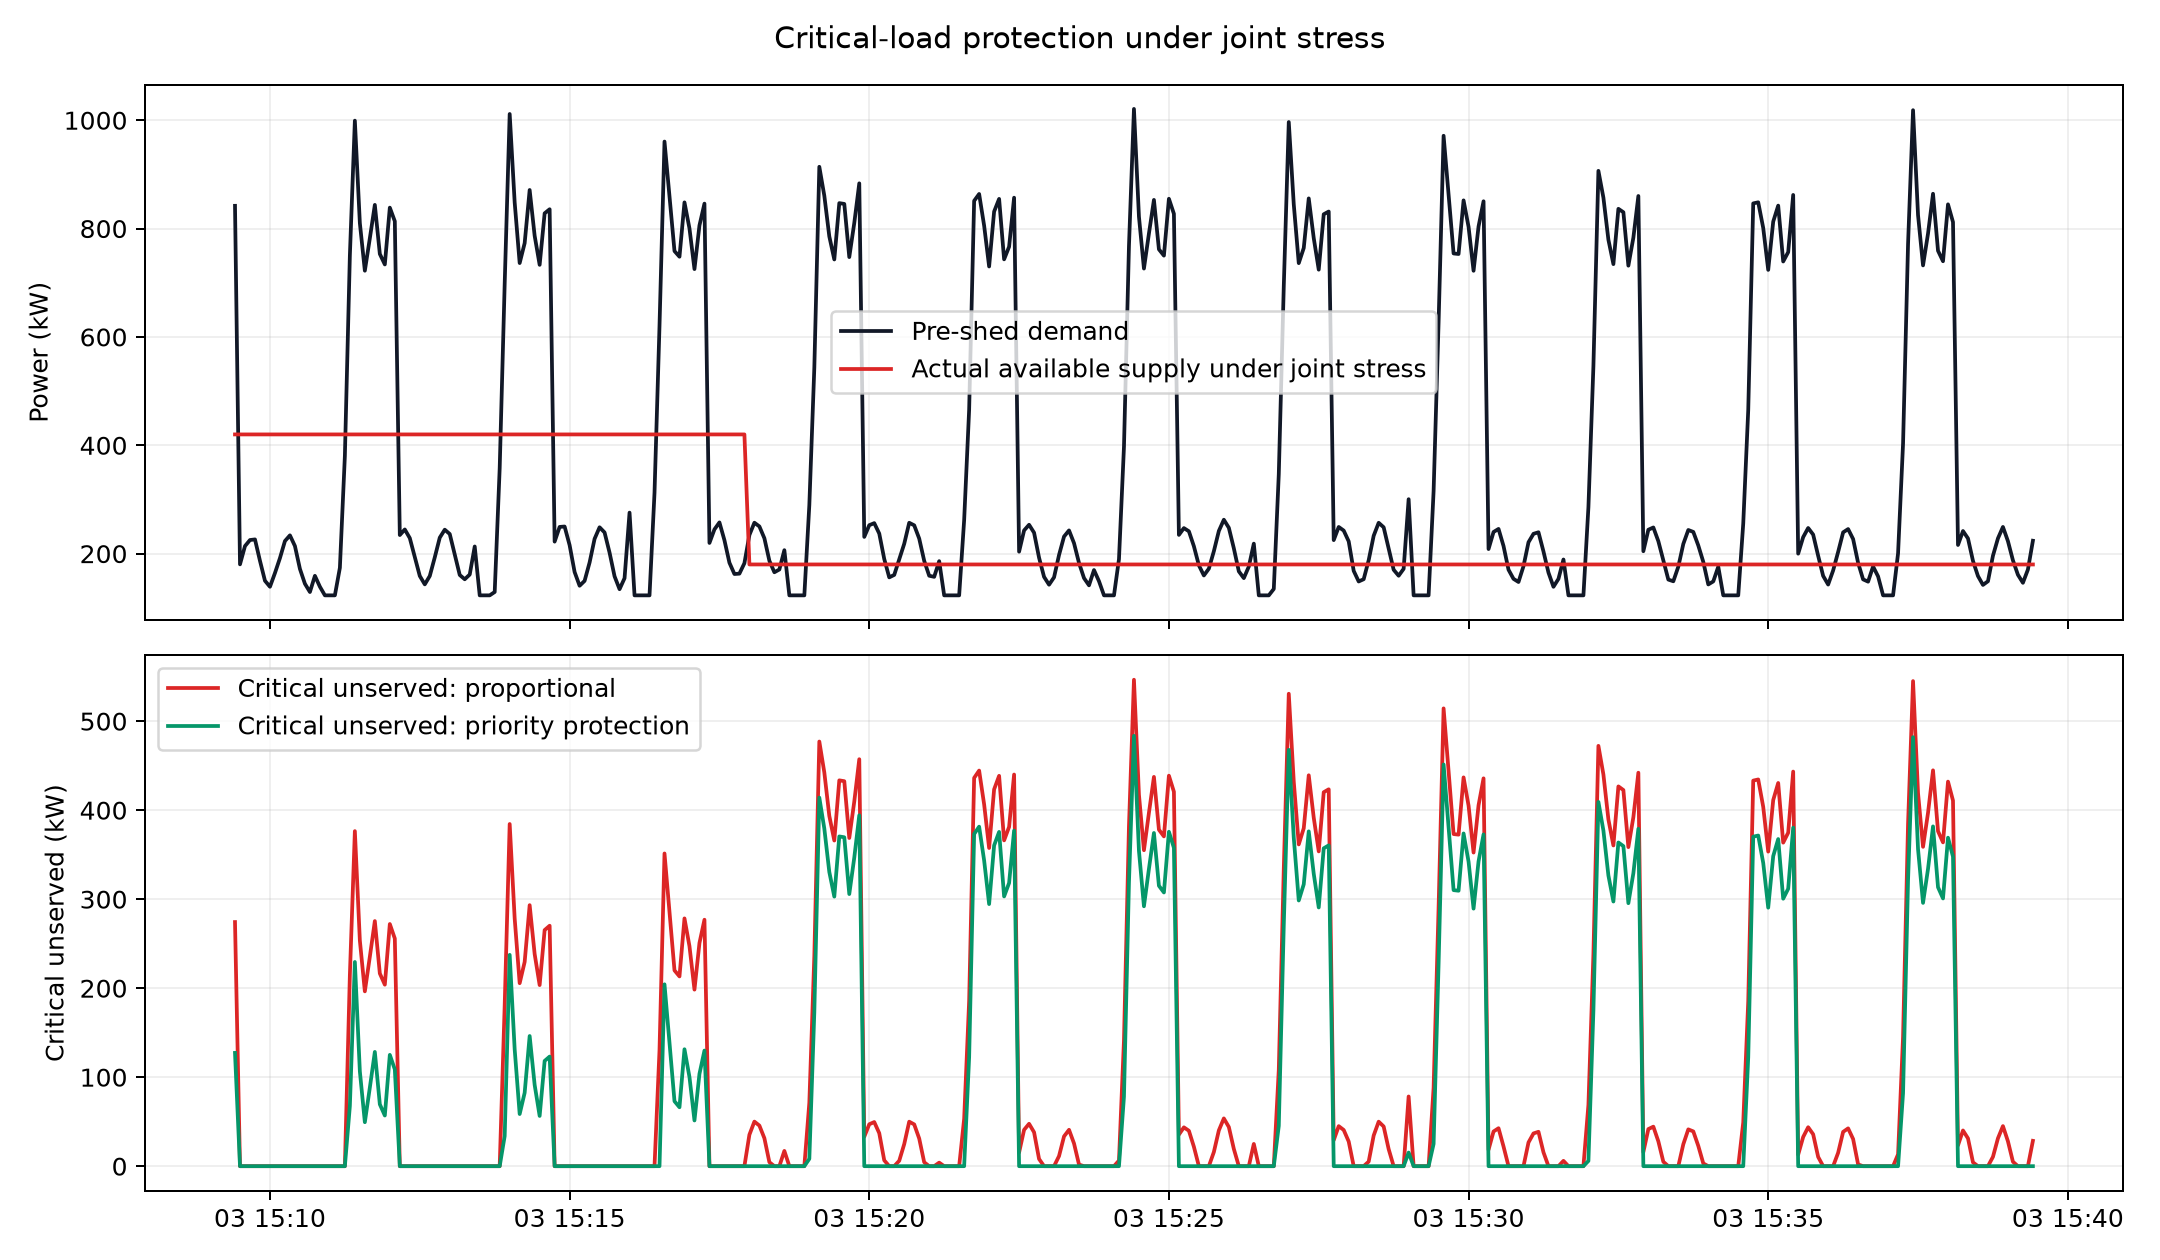
\includegraphics[width=\linewidth,keepaspectratio]{../figures/fig07_joint_stress_critical_protection.png}
\caption{Critical-load protection under joint stress}
\label{fig:joint-stress-protection}
\end{figure}

\section{Discussion}\label{discussion}

\subsection{Energy-system performance}\label{energy-system-performance}

Within the ten simulated holdouts, RSS reduces unserved energy and its
shortage-dominated composite cost relative to the prespecified baselines.
Relative to RB, it reduces unserved energy by 3.27\%, risk-adjusted cost by
3.85\%, and diesel use by 37.20 L. Relative to MLR, it reduces unserved energy
by 10.22\% and risk-adjusted cost by 9.34\%, while using 2.61 L more diesel.
Risk-adjusted cost is not an independent economic outcome. The controller
therefore favors supply continuity when forecast transitions and reserve
constraints make a small increase in fuel use preferable to additional
shortage. All main-comparison trajectories satisfy the power-balance,
equipment-capacity, commitment, and SOC checks; intervention audit scopes are
reported with their respective analyses.

The forecasting results show that average prediction accuracy alone is an
incomplete characterization for this application. iTransformer gives the lowest
overall error, while transition-specific errors are reported separately because
rapid load changes enter generator-commitment and reserve decisions. The
scenario envelope carries this uncertainty into the dispatch problem instead of
relying on a single point forecast.

\subsection{Operating mechanisms}\label{operating-mechanisms}

Two prespecified component interventions are associated with lower unserved
energy within the simulated protocol. First, enabling the implemented forecast-
envelope bundle is associated with a 2.12 kWh mean reduction per holdout in the
paired RSS-centered intervention. Second, activating the SOC supervisor is
associated with a 2.86--4.11 kWh mean reduction per holdout in the specified
SC/RAC-centered contrasts. The controller rules provide a consistent operational
interpretation: they prepare reachable generator capacity before the battery
reaches its lower operating region and avoid releasing protection immediately
after a short recovery.

The adaptive risk signal has no marginal aggregate-shortage effect in the
specified intervention. In the auxiliary studies, the raw evidential variant
improves selected classification metrics while worsening the Brier score, and
temperature calibration improves the Brier score in a separate holdout group;
neither changes unserved energy. These results narrow the role of the risk
interface to separately reported operator-facing information. The forecast-
envelope bundle and reserve--SOC logic are associated with reductions in their
corresponding interventions. Likewise, priority-based allocation protects
critical loads during severe disturbances but cannot reduce total shortage when
aggregate supply is fixed. These results are not an additive decomposition of
the RSS--RB, RSS--MLR, or RSS--CR differences.

\subsection{Engineering applicability}\label{engineering-applicability}

Earlier drilling rig studies established the value of rule-based generator
scheduling and battery storage. The present framework adds forecast
uncertainty, discrete multi-generator constraints, explicit storage reserve,
and priority-based protection in a single rolling controller. The resulting
structure may offer a transferable control architecture for other industrial
grid--diesel--battery systems with abrupt loads and limited grid capacity, but
such transfer requires system-specific model identification, parameterization,
safety approval, and validation.

Deployment requires synchronized total active power, individual generator
states and outputs, battery SOC and power, grid capacity measurements, fuel
consumption, energy prices, and approved load classes. Equipment ramp limits,
minimum up/down times, efficiency curves, startup costs, degradation costs,
and terminal SOC requirements should be replaced with site values. The next
validation step is an external replay with site data followed by
hardware-in-the-loop testing on the intended control platform.

\section{Limitations and reproducibility}\label{limitations-and-reproducibility}

The evaluation record is generated by one mechanistic simulation parameterized
from public evidence; synchronized target-rig electrical measurements were not
available. The ten holdouts test controller behavior across independently
generated cases but do not capture installation-specific equipment dynamics,
communication delays, or operator actions. The forecasting comparison also
uses a fixed retrospective replay rather than an external prospective dataset.
The holdouts are pseudorandom realizations of the same frozen simulator, not
samples from an empirically fitted target-rig population. The seven forecast
members likewise are deterministic model-disagreement trajectories rather than
probability-calibrated samples; with their equal weights, the reported CVaR
levels select the same worst member and do not establish probabilistic coverage.

The bundled causal full-MILP boundary comparator omits the forecast envelope and
supervisory policy, while the perfect-foresight solution is available only for
the original two cases. These references compare different declared information
and control bundles and do not support attribution to any single component;
they also do not exhaust all possible robust or stochastic optimization
baselines. The emergency load classes and equipment parameters also require
site-specific approval and calibration.

The source artifacts, configurations, result manifests, and analysis scripts
are versioned locally. A public release of the permitted data generator and
reproducibility package should accompany the final article or be deposited in
a suitable repository.

\section{Conclusions}\label{conclusions}

This study evaluated reserve--SOC supervisory energy management using a 72 h
record and ten independently generated holdouts from a single mechanistic
drilling-load and power-system simulator; no synchronized measurements from
the target rig were used. Seven online controllers shared the simulated plant,
realized traces, price terms, execution layer, and audit path; their forecast
representations and terminal-SOC rules followed their declared controller-
specific definitions.

Across ten holdouts, RSS reduces unserved energy by 3.27\% relative to
rule-based control, 10.22\% relative to deterministic margin-loaded reference
MPC (MLR), and 30.23\% relative to the causal full-MILP boundary comparator.
Risk-adjusted cost falls by 3.85\% relative to rule-based control and 9.34\%
relative to MLR; these shortage-dominated composite cost comparisons are not
independent economic evidence. The causal full-MILP is independently
implemented, uses a single point forecast, and
omits both the forecast-error envelope and reserve--SOC supervisor. Because it
is weaker than rule-based control under this protocol, the 30.23\% RSS--CR gap
is a bundled boundary comparison rather than being attributable to any single
component or a like-for-like ablation. Component-level interventions associate
the forecast-envelope bundle and SOC supervision with local reductions in their
corresponding interventions, while the adaptive risk signal in the specified
intervention has no marginal shortage effect. All main-comparison trajectories
satisfy the stated physical
constraints, and the maximum recorded decision time is 0.36 s.

Within this simulated system, the results support coordinating storage reserve
with forecast uncertainty and reachable generator capacity during rapid load
transitions. They do not establish performance for the target rig or for
drilling rigs generally. Site-specific electrical data and hardware-in-the-loop
testing remain necessary before field-performance conclusions can be drawn.


\section*{CRediT authorship contribution statement}
\noindent\textbf{Shixing Zhang}: Conceptualization, Methodology, Software,
Formal analysis, Investigation, Visualization, Writing--original draft, Project
administration.\\
\textbf{Pengchong Wei}: Methodology, Validation, Investigation, Data curation,
Writing--review \& editing.\\
\textbf{Lei Luo}: Resources, Validation, Writing--review \& editing.\\
\textbf{Pengfei Zhang}: Investigation, Validation, Writing--review \& editing.\\
\textbf{Xingjun Yu}: Supervision, Project administration, Funding acquisition,
Resources, Writing--review \& editing.

\section*{Declaration of competing interest}
All authors are employees of companies affiliated with China National Petroleum
Corporation (CNPC). This work was supported by the CNPC Youth Science and
Technology Special Project (Project No.~2026DQ03150). The funder had no role in
the study design, data generation, analysis and interpretation, manuscript
preparation, or the decision to submit the article. The authors declare no other
competing financial interests or personal relationships that could have
influenced the work reported in this paper.

\section*{Data availability}
The compact reproducibility package is available in the public GitHub repository
at \url{https://github.com/shixingzhang1994-byte/rig-energy-forecasting/tree/reproducibility-package-v1}.
It contains the permitted mechanistic simulator and data generator, controller
and experiment configurations, environment specification, the simulated 72~h
record, selected trajectory-level audit outputs, result manifests, analysis
scripts, and manuscript sources supporting the reported comparisons. Large
development intermediates, duplicate plots, and model weights are excluded as
documented in the repository README. A DOI-bearing archival release and its
reuse license will be added after author and institutional confirmation.

\section*{Acknowledgements}
This work was carried out under the China National Petroleum Corporation
(CNPC) Youth Science and Technology Special Project (Project
No.~2026DQ03150).

\bibliographystyle{elsarticle-num}
\bibliography{refs}

\end{document}
